\documentclass{article}
\usepackage{url,color,xspace,verbatim,subfig,ctable,multirow,listings}
\usepackage[utf8]{inputenc}
\usepackage[T1]{fontenc}
\usepackage{txfonts}
\usepackage{rotating}
\usepackage{paralist}
\usepackage{subfig}
\usepackage{graphics}
\usepackage{enumitem}
\usepackage{times}
\usepackage{amssymb}
\usepackage[colorlinks=true]{hyperref}
\usepackage[ruled,vlined]{algorithm2e}
\usepackage[toc,page]{appendix}
% ==================================================

\graphicspath{{figs/}}
\urlstyle{sf}

% tikz stuff
\usepackage{tikz}
\usepackage{pgfplots}
% configuration
\usetikzlibrary{shapes,positioning,calc,snakes,arrows,shapes,fit,backgrounds}
\pgfplotsset{width=.9\linewidth}

\lstset{
  language=C,
  basicstyle=\ttfamily \small,
  flexiblecolumns=false,
  basewidth={0.5em,0.45em},
  boxpos=t,
}

\newcommand{\etal}{{\it et al.}\xspace}
\newcommand{\naive}{na\"{\i}ve\xspace}
\newcommand{\Naive}{Na\"{\i}ve\xspace}
\newcommand{\textc}[1]{{\color{gray} {\footnotesize #1}}}

\definecolor{skRed}{RGB}{155,25,25}
\newcommand{\stefan}[1]{
  {\color{skRed}[{\color{red}{SK}} #1]}}

\setcounter{section}{0} % Start sections with 1, not 0
\begin{document}

\title{Adaptive broadcast tree for multicores}

% email address
\newcommand{\eaddr}{stefan.kaestle@inf.ethz.ch}
\newcommand{\email}{\href{mailto:\eaddr}{\eaddr}}

\author{Stefan Kaestle\\
  \email \\
  Systems Group, ETH Zurich}

\maketitle

% keywords: modeling, simulation, overlay networks, scheduling

%%%%%%%%%%%%%%%%%%%%%%%%%%%%%%%%%%%%%%%%%%%%%%%%%%
%%%%%%%%%%%%%%%%%%%%%%%%%%%%%%%%%%%%%%%%%%%%%%%%%%
\section{Visualization}

\section{Topologies}
\newpage
\subsection{ziger1}
\newpage
\subsubsection{badtree}
\begin{tikzpicture}[]
  % Insert visualization
  \input{graphs/visu_ziger1_badtree}
\end{tikzpicture}
\newpage
\subsubsection{cluster}
\begin{tikzpicture}[]
  % Insert visualization
  \input{graphs/visu_ziger1_cluster}
\end{tikzpicture}
\newpage
\subsubsection{mst}
\begin{tikzpicture}[]
  % Insert visualization
  \input{graphs/visu_ziger1_mst}
\end{tikzpicture}
\newpage
\subsubsection{bintree}
\begin{tikzpicture}[]
  % Insert visualization
  \input{graphs/visu_ziger1_bintree}
\end{tikzpicture}
\newpage
\subsubsection{sequential}
\begin{tikzpicture}[]
  % Insert visualization
  \input{graphs/visu_ziger1_sequential}
\end{tikzpicture}
\newpage
\subsubsection{ring}
\begin{tikzpicture}[]
  % Insert visualization
  \input{graphs/visu_ziger1_ring}
\end{tikzpicture}
\newpage
\subsection{gruyere}
\newpage
\subsubsection{badtree}
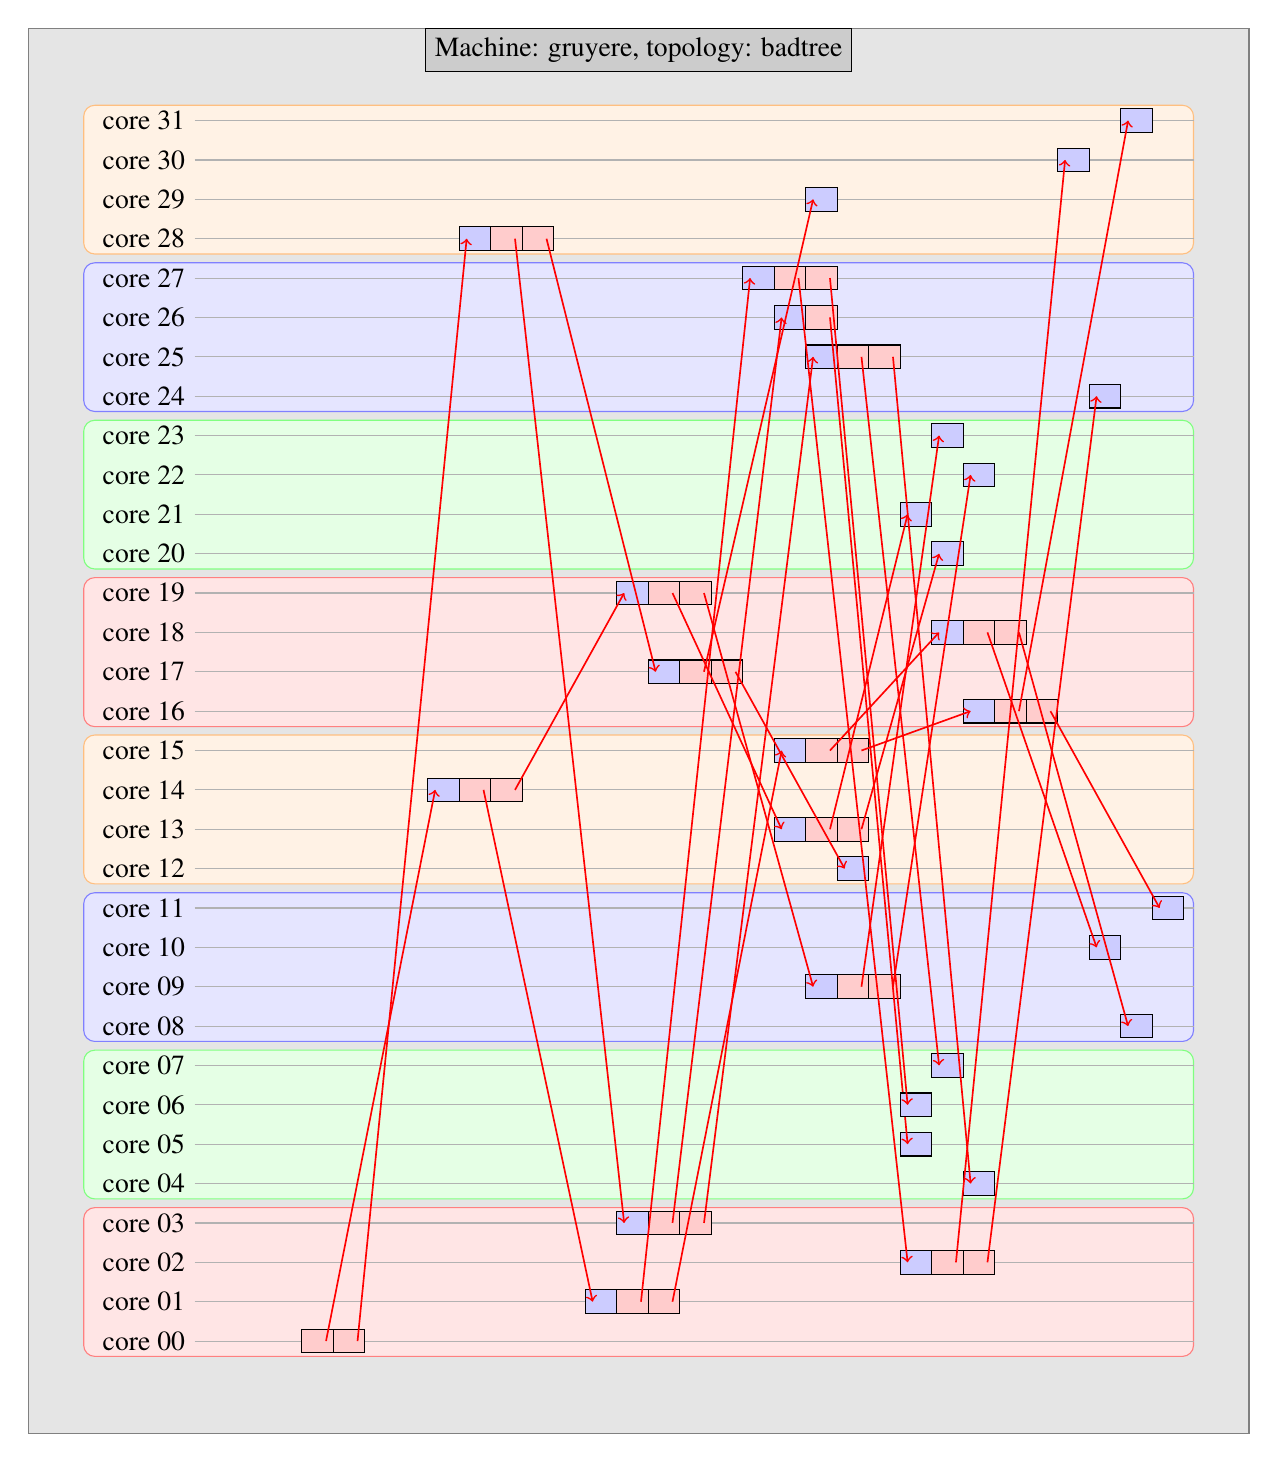
\begin{tikzpicture}[]
  % Insert visualization
  \node (core_0_label) at (0mm,0mm) {core 00};
\node (core_1_label) at (0mm,5mm) {core 01};
\node (core_2_label) at (0mm,10mm) {core 02};
\node (core_3_label) at (0mm,15mm) {core 03};
\node (core_4_label) at (0mm,20mm) {core 04};
\node (core_5_label) at (0mm,25mm) {core 05};
\node (core_6_label) at (0mm,30mm) {core 06};
\node (core_7_label) at (0mm,35mm) {core 07};
\node (core_8_label) at (0mm,40mm) {core 08};
\node (core_9_label) at (0mm,45mm) {core 09};
\node (core_10_label) at (0mm,50mm) {core 10};
\node (core_11_label) at (0mm,55mm) {core 11};
\node (core_12_label) at (0mm,60mm) {core 12};
\node (core_13_label) at (0mm,65mm) {core 13};
\node (core_14_label) at (0mm,70mm) {core 14};
\node (core_15_label) at (0mm,75mm) {core 15};
\node (core_16_label) at (0mm,80mm) {core 16};
\node (core_17_label) at (0mm,85mm) {core 17};
\node (core_18_label) at (0mm,90mm) {core 18};
\node (core_19_label) at (0mm,95mm) {core 19};
\node (core_20_label) at (0mm,100mm) {core 20};
\node (core_21_label) at (0mm,105mm) {core 21};
\node (core_22_label) at (0mm,110mm) {core 22};
\node (core_23_label) at (0mm,115mm) {core 23};
\node (core_24_label) at (0mm,120mm) {core 24};
\node (core_25_label) at (0mm,125mm) {core 25};
\node (core_26_label) at (0mm,130mm) {core 26};
\node (core_27_label) at (0mm,135mm) {core 27};
\node (core_28_label) at (0mm,140mm) {core 28};
\node (core_29_label) at (0mm,145mm) {core 29};
\node (core_30_label) at (0mm,150mm) {core 30};
\node (core_31_label) at (0mm,155mm) {core 31};
\node[draw,fill=red!20,minimum width=4mm, minimum height=3mm,anchor=west] (s_0_14) at (20mm,0mm) {};
\node[draw,fill=red!20,minimum width=4mm, minimum height=3mm,anchor=west] (s_0_28) at (24mm,0mm) {};
\node[draw,fill=blue!20,minimum width=4mm, minimum height=3mm,anchor=west] (r_0_14) at (36mm,70mm) {};
\draw[->,semithick,color=red] ($(s_0_14.east)-(1mm,0mm)$) -- ($(r_0_14.west)+(1mm,0mm)$); 
\node[draw,fill=red!20,minimum width=4mm, minimum height=3mm,anchor=west] (s_14_1) at (40mm,70mm) {};
\node[draw,fill=red!20,minimum width=4mm, minimum height=3mm,anchor=west] (s_14_19) at (44mm,70mm) {};
\node[draw,fill=blue!20,minimum width=4mm, minimum height=3mm,anchor=west] (r_0_28) at (40mm,140mm) {};
\draw[->,semithick,color=red] ($(s_0_28.east)-(1mm,0mm)$) -- ($(r_0_28.west)+(1mm,0mm)$); 
\node[draw,fill=red!20,minimum width=4mm, minimum height=3mm,anchor=west] (s_28_3) at (44mm,140mm) {};
\node[draw,fill=red!20,minimum width=4mm, minimum height=3mm,anchor=west] (s_28_17) at (48mm,140mm) {};
\node[draw,fill=blue!20,minimum width=4mm, minimum height=3mm,anchor=west] (r_14_1) at (56mm,5mm) {};
\draw[->,semithick,color=red] ($(s_14_1.east)-(1mm,0mm)$) -- ($(r_14_1.west)+(1mm,0mm)$); 
\node[draw,fill=red!20,minimum width=4mm, minimum height=3mm,anchor=west] (s_1_27) at (60mm,5mm) {};
\node[draw,fill=red!20,minimum width=4mm, minimum height=3mm,anchor=west] (s_1_15) at (64mm,5mm) {};
\node[draw,fill=blue!20,minimum width=4mm, minimum height=3mm,anchor=west] (r_28_3) at (60mm,15mm) {};
\draw[->,semithick,color=red] ($(s_28_3.east)-(1mm,0mm)$) -- ($(r_28_3.west)+(1mm,0mm)$); 
\node[draw,fill=red!20,minimum width=4mm, minimum height=3mm,anchor=west] (s_3_26) at (64mm,15mm) {};
\node[draw,fill=red!20,minimum width=4mm, minimum height=3mm,anchor=west] (s_3_25) at (68mm,15mm) {};
\node[draw,fill=blue!20,minimum width=4mm, minimum height=3mm,anchor=west] (r_14_19) at (60mm,95mm) {};
\draw[->,semithick,color=red] ($(s_14_19.east)-(1mm,0mm)$) -- ($(r_14_19.west)+(1mm,0mm)$); 
\node[draw,fill=red!20,minimum width=4mm, minimum height=3mm,anchor=west] (s_19_13) at (64mm,95mm) {};
\node[draw,fill=red!20,minimum width=4mm, minimum height=3mm,anchor=west] (s_19_9) at (68mm,95mm) {};
\node[draw,fill=blue!20,minimum width=4mm, minimum height=3mm,anchor=west] (r_28_17) at (64mm,85mm) {};
\draw[->,semithick,color=red] ($(s_28_17.east)-(1mm,0mm)$) -- ($(r_28_17.west)+(1mm,0mm)$); 
\node[draw,fill=red!20,minimum width=4mm, minimum height=3mm,anchor=west] (s_17_29) at (68mm,85mm) {};
\node[draw,fill=red!20,minimum width=4mm, minimum height=3mm,anchor=west] (s_17_12) at (72mm,85mm) {};
\node[draw,fill=blue!20,minimum width=4mm, minimum height=3mm,anchor=west] (r_1_27) at (76mm,135mm) {};
\draw[->,semithick,color=red] ($(s_1_27.east)-(1mm,0mm)$) -- ($(r_1_27.west)+(1mm,0mm)$); 
\node[draw,fill=red!20,minimum width=4mm, minimum height=3mm,anchor=west] (s_27_2) at (80mm,135mm) {};
\node[draw,fill=red!20,minimum width=4mm, minimum height=3mm,anchor=west] (s_27_6) at (84mm,135mm) {};
\node[draw,fill=blue!20,minimum width=4mm, minimum height=3mm,anchor=west] (r_19_13) at (80mm,65mm) {};
\draw[->,semithick,color=red] ($(s_19_13.east)-(1mm,0mm)$) -- ($(r_19_13.west)+(1mm,0mm)$); 
\node[draw,fill=red!20,minimum width=4mm, minimum height=3mm,anchor=west] (s_13_21) at (84mm,65mm) {};
\node[draw,fill=red!20,minimum width=4mm, minimum height=3mm,anchor=west] (s_13_20) at (88mm,65mm) {};
\node[draw,fill=blue!20,minimum width=4mm, minimum height=3mm,anchor=west] (r_1_15) at (80mm,75mm) {};
\draw[->,semithick,color=red] ($(s_1_15.east)-(1mm,0mm)$) -- ($(r_1_15.west)+(1mm,0mm)$); 
\node[draw,fill=red!20,minimum width=4mm, minimum height=3mm,anchor=west] (s_15_18) at (84mm,75mm) {};
\node[draw,fill=red!20,minimum width=4mm, minimum height=3mm,anchor=west] (s_15_16) at (88mm,75mm) {};
\node[draw,fill=blue!20,minimum width=4mm, minimum height=3mm,anchor=west] (r_3_26) at (80mm,130mm) {};
\draw[->,semithick,color=red] ($(s_3_26.east)-(1mm,0mm)$) -- ($(r_3_26.west)+(1mm,0mm)$); 
\node[draw,fill=red!20,minimum width=4mm, minimum height=3mm,anchor=west] (s_26_5) at (84mm,130mm) {};
\node[draw,fill=blue!20,minimum width=4mm, minimum height=3mm,anchor=west] (r_19_9) at (84mm,45mm) {};
\draw[->,semithick,color=red] ($(s_19_9.east)-(1mm,0mm)$) -- ($(r_19_9.west)+(1mm,0mm)$); 
\node[draw,fill=red!20,minimum width=4mm, minimum height=3mm,anchor=west] (s_9_23) at (88mm,45mm) {};
\node[draw,fill=red!20,minimum width=4mm, minimum height=3mm,anchor=west] (s_9_22) at (92mm,45mm) {};
\node[draw,fill=blue!20,minimum width=4mm, minimum height=3mm,anchor=west] (r_17_29) at (84mm,145mm) {};
\draw[->,semithick,color=red] ($(s_17_29.east)-(1mm,0mm)$) -- ($(r_17_29.west)+(1mm,0mm)$); 
\node[draw,fill=blue!20,minimum width=4mm, minimum height=3mm,anchor=west] (r_3_25) at (84mm,125mm) {};
\draw[->,semithick,color=red] ($(s_3_25.east)-(1mm,0mm)$) -- ($(r_3_25.west)+(1mm,0mm)$); 
\node[draw,fill=red!20,minimum width=4mm, minimum height=3mm,anchor=west] (s_25_7) at (88mm,125mm) {};
\node[draw,fill=red!20,minimum width=4mm, minimum height=3mm,anchor=west] (s_25_4) at (92mm,125mm) {};
\node[draw,fill=blue!20,minimum width=4mm, minimum height=3mm,anchor=west] (r_17_12) at (88mm,60mm) {};
\draw[->,semithick,color=red] ($(s_17_12.east)-(1mm,0mm)$) -- ($(r_17_12.west)+(1mm,0mm)$); 
\node[draw,fill=blue!20,minimum width=4mm, minimum height=3mm,anchor=west] (r_26_5) at (96mm,25mm) {};
\draw[->,semithick,color=red] ($(s_26_5.east)-(1mm,0mm)$) -- ($(r_26_5.west)+(1mm,0mm)$); 
\node[draw,fill=blue!20,minimum width=4mm, minimum height=3mm,anchor=west] (r_13_21) at (96mm,105mm) {};
\draw[->,semithick,color=red] ($(s_13_21.east)-(1mm,0mm)$) -- ($(r_13_21.west)+(1mm,0mm)$); 
\node[draw,fill=blue!20,minimum width=4mm, minimum height=3mm,anchor=west] (r_27_6) at (96mm,30mm) {};
\draw[->,semithick,color=red] ($(s_27_6.east)-(1mm,0mm)$) -- ($(r_27_6.west)+(1mm,0mm)$); 
\node[draw,fill=blue!20,minimum width=4mm, minimum height=3mm,anchor=west] (r_27_2) at (96mm,10mm) {};
\draw[->,semithick,color=red] ($(s_27_2.east)-(1mm,0mm)$) -- ($(r_27_2.west)+(1mm,0mm)$); 
\node[draw,fill=red!20,minimum width=4mm, minimum height=3mm,anchor=west] (s_2_30) at (100mm,10mm) {};
\node[draw,fill=red!20,minimum width=4mm, minimum height=3mm,anchor=west] (s_2_24) at (104mm,10mm) {};
\node[draw,fill=blue!20,minimum width=4mm, minimum height=3mm,anchor=west] (r_9_23) at (100mm,115mm) {};
\draw[->,semithick,color=red] ($(s_9_23.east)-(1mm,0mm)$) -- ($(r_9_23.west)+(1mm,0mm)$); 
\node[draw,fill=blue!20,minimum width=4mm, minimum height=3mm,anchor=west] (r_15_18) at (100mm,90mm) {};
\draw[->,semithick,color=red] ($(s_15_18.east)-(1mm,0mm)$) -- ($(r_15_18.west)+(1mm,0mm)$); 
\node[draw,fill=red!20,minimum width=4mm, minimum height=3mm,anchor=west] (s_18_10) at (104mm,90mm) {};
\node[draw,fill=red!20,minimum width=4mm, minimum height=3mm,anchor=west] (s_18_8) at (108mm,90mm) {};
\node[draw,fill=blue!20,minimum width=4mm, minimum height=3mm,anchor=west] (r_13_20) at (100mm,100mm) {};
\draw[->,semithick,color=red] ($(s_13_20.east)-(1mm,0mm)$) -- ($(r_13_20.west)+(1mm,0mm)$); 
\node[draw,fill=blue!20,minimum width=4mm, minimum height=3mm,anchor=west] (r_25_7) at (100mm,35mm) {};
\draw[->,semithick,color=red] ($(s_25_7.east)-(1mm,0mm)$) -- ($(r_25_7.west)+(1mm,0mm)$); 
\node[draw,fill=blue!20,minimum width=4mm, minimum height=3mm,anchor=west] (r_25_4) at (104mm,20mm) {};
\draw[->,semithick,color=red] ($(s_25_4.east)-(1mm,0mm)$) -- ($(r_25_4.west)+(1mm,0mm)$); 
\node[draw,fill=blue!20,minimum width=4mm, minimum height=3mm,anchor=west] (r_9_22) at (104mm,110mm) {};
\draw[->,semithick,color=red] ($(s_9_22.east)-(1mm,0mm)$) -- ($(r_9_22.west)+(1mm,0mm)$); 
\node[draw,fill=blue!20,minimum width=4mm, minimum height=3mm,anchor=west] (r_15_16) at (104mm,80mm) {};
\draw[->,semithick,color=red] ($(s_15_16.east)-(1mm,0mm)$) -- ($(r_15_16.west)+(1mm,0mm)$); 
\node[draw,fill=red!20,minimum width=4mm, minimum height=3mm,anchor=west] (s_16_31) at (108mm,80mm) {};
\node[draw,fill=red!20,minimum width=4mm, minimum height=3mm,anchor=west] (s_16_11) at (112mm,80mm) {};
\node[draw,fill=blue!20,minimum width=4mm, minimum height=3mm,anchor=west] (r_2_30) at (116mm,150mm) {};
\draw[->,semithick,color=red] ($(s_2_30.east)-(1mm,0mm)$) -- ($(r_2_30.west)+(1mm,0mm)$); 
\node[draw,fill=blue!20,minimum width=4mm, minimum height=3mm,anchor=west] (r_2_24) at (120mm,120mm) {};
\draw[->,semithick,color=red] ($(s_2_24.east)-(1mm,0mm)$) -- ($(r_2_24.west)+(1mm,0mm)$); 
\node[draw,fill=blue!20,minimum width=4mm, minimum height=3mm,anchor=west] (r_18_10) at (120mm,50mm) {};
\draw[->,semithick,color=red] ($(s_18_10.east)-(1mm,0mm)$) -- ($(r_18_10.west)+(1mm,0mm)$); 
\node[draw,fill=blue!20,minimum width=4mm, minimum height=3mm,anchor=west] (r_18_8) at (124mm,40mm) {};
\draw[->,semithick,color=red] ($(s_18_8.east)-(1mm,0mm)$) -- ($(r_18_8.west)+(1mm,0mm)$); 
\node[draw,fill=blue!20,minimum width=4mm, minimum height=3mm,anchor=west] (r_16_31) at (124mm,155mm) {};
\draw[->,semithick,color=red] ($(s_16_31.east)-(1mm,0mm)$) -- ($(r_16_31.west)+(1mm,0mm)$); 
\node[draw,fill=blue!20,minimum width=4mm, minimum height=3mm,anchor=west] (r_16_11) at (128mm,55mm) {};
\draw[->,semithick,color=red] ($(s_16_11.east)-(1mm,0mm)$) -- ($(r_16_11.west)+(1mm,0mm)$); 
\begin{pgfonlayer}{background}
\node [fit=(core_0_label) (core_1_label) (core_2_label) (core_3_label) (core_4_label) (core_5_label) (core_6_label) (core_7_label) (core_8_label) (core_9_label) (core_10_label) (core_11_label) (core_12_label) (core_13_label) (core_14_label) (core_15_label) (core_16_label) (core_17_label) (core_18_label) (core_19_label) (core_20_label) (core_21_label) (core_22_label) (core_23_label) (core_24_label) (core_25_label) (core_26_label) (core_27_label) (core_28_label) (core_29_label) (core_30_label) (core_31_label) (s_0_14) (s_0_28) (r_0_14) (s_14_1) (s_14_19) (r_0_28) (s_28_3) (s_28_17) (r_14_1) (s_1_27) (s_1_15) (r_14_19) (s_19_13) (s_19_9) (r_28_3) (s_3_26) (s_3_25) (r_28_17) (s_17_29) (s_17_12) (r_1_27) (s_27_2) (s_27_6) (r_3_26) (s_26_5) (r_1_15) (s_15_18) (s_15_16) (r_19_13) (s_13_21) (s_13_20) (r_3_25) (s_25_7) (s_25_4) (r_17_29) (r_19_9) (s_9_23) (s_9_22) (r_17_12) (r_27_2) (s_2_30) (s_2_24) (r_13_21) (r_27_6) (r_26_5) (r_13_20) (r_25_7) (r_15_18) (s_18_10) (s_18_8) (r_9_23) (r_25_4) (r_15_16) (s_16_31) (s_16_11) (r_9_22) (r_2_30) (r_18_10) (r_2_24) (r_18_8) (r_16_31) (r_16_11) (core_0_label) (core_1_label) (core_2_label) (core_3_label) (core_4_label) (core_5_label) (core_6_label) (core_7_label) (core_8_label) (core_9_label) (core_10_label) (core_11_label) (core_12_label) (core_13_label) (core_14_label) (core_15_label) (core_16_label) (core_17_label) (core_18_label) (core_19_label) (core_20_label) (core_21_label) (core_22_label) (core_23_label) (core_24_label) (core_25_label) (core_26_label) (core_27_label) (core_28_label) (core_29_label) (core_30_label) (core_31_label) (s_0_14) (s_0_28) (r_0_14) (s_14_1) (s_14_19) (r_0_28) (s_28_3) (s_28_17) (r_14_1) (s_1_27) (s_1_15) (r_28_3) (s_3_26) (s_3_25) (r_14_19) (s_19_13) (s_19_9) (r_28_17) (s_17_29) (s_17_12) (r_1_27) (s_27_2) (s_27_6) (r_19_13) (s_13_21) (s_13_20) (r_1_15) (s_15_18) (s_15_16) (r_3_26) (s_26_5) (r_19_9) (s_9_23) (s_9_22) (r_17_29) (r_3_25) (s_25_7) (s_25_4) (r_17_12) (r_26_5) (r_13_21) (r_27_6) (r_27_2) (s_2_30) (s_2_24) (r_9_23) (r_15_18) (s_18_10) (s_18_8) (r_13_20) (r_25_7) (r_25_4) (r_9_22) (r_15_16) (s_16_31) (s_16_11) (r_2_30) (r_2_24) (r_18_10) (r_18_8) (r_16_31) (r_16_11)] (allobjects) {};
\node [draw=black!50,fill=black!10,fit=(core_0_label) (core_1_label) (core_2_label) (core_3_label) (core_4_label) (core_5_label) (core_6_label) (core_7_label) (core_8_label) (core_9_label) (core_10_label) (core_11_label) (core_12_label) (core_13_label) (core_14_label) (core_15_label) (core_16_label) (core_17_label) (core_18_label) (core_19_label) (core_20_label) (core_21_label) (core_22_label) (core_23_label) (core_24_label) (core_25_label) (core_26_label) (core_27_label) (core_28_label) (core_29_label) (core_30_label) (core_31_label) (s_0_14) (s_0_28) (r_0_14) (s_14_1) (s_14_19) (r_0_28) (s_28_3) (s_28_17) (r_14_1) (s_1_27) (s_1_15) (r_14_19) (s_19_13) (s_19_9) (r_28_3) (s_3_26) (s_3_25) (r_28_17) (s_17_29) (s_17_12) (r_1_27) (s_27_2) (s_27_6) (r_3_26) (s_26_5) (r_1_15) (s_15_18) (s_15_16) (r_19_13) (s_13_21) (s_13_20) (r_3_25) (s_25_7) (s_25_4) (r_17_29) (r_19_9) (s_9_23) (s_9_22) (r_17_12) (r_27_2) (s_2_30) (s_2_24) (r_13_21) (r_27_6) (r_26_5) (r_13_20) (r_25_7) (r_15_18) (s_18_10) (s_18_8) (r_9_23) (r_25_4) (r_15_16) (s_16_31) (s_16_11) (r_9_22) (r_2_30) (r_18_10) (r_2_24) (r_18_8) (r_16_31) (r_16_11) (core_0_label) (core_1_label) (core_2_label) (core_3_label) (core_4_label) (core_5_label) (core_6_label) (core_7_label) (core_8_label) (core_9_label) (core_10_label) (core_11_label) (core_12_label) (core_13_label) (core_14_label) (core_15_label) (core_16_label) (core_17_label) (core_18_label) (core_19_label) (core_20_label) (core_21_label) (core_22_label) (core_23_label) (core_24_label) (core_25_label) (core_26_label) (core_27_label) (core_28_label) (core_29_label) (core_30_label) (core_31_label) (s_0_14) (s_0_28) (r_0_14) (s_14_1) (s_14_19) (r_0_28) (s_28_3) (s_28_17) (r_14_1) (s_1_27) (s_1_15) (r_28_3) (s_3_26) (s_3_25) (r_14_19) (s_19_13) (s_19_9) (r_28_17) (s_17_29) (s_17_12) (r_1_27) (s_27_2) (s_27_6) (r_19_13) (s_13_21) (s_13_20) (r_1_15) (s_15_18) (s_15_16) (r_3_26) (s_26_5) (r_19_9) (s_9_23) (s_9_22) (r_17_29) (r_3_25) (s_25_7) (s_25_4) (r_17_12) (r_26_5) (r_13_21) (r_27_6) (r_27_2) (s_2_30) (s_2_24) (r_9_23) (r_15_18) (s_18_10) (s_18_8) (r_13_20) (r_25_7) (r_25_4) (r_9_22) (r_15_16) (s_16_31) (s_16_11) (r_2_30) (r_2_24) (r_18_10) (r_18_8) (r_16_31) (r_16_11),scale=1.1] (bg) {};
\draw let \p1 = (allobjects.east) in node[] (numa_axis_0) at (\x1,0mm) {};
\draw let \p1 = (allobjects.east) in node[] (numa_axis_1) at (\x1,5mm) {};
\draw let \p1 = (allobjects.east) in node[] (numa_axis_2) at (\x1,10mm) {};
\draw let \p1 = (allobjects.east) in node[] (numa_axis_3) at (\x1,15mm) {};
\draw let \p1 = (allobjects.east) in node[] (numa_axis_4) at (\x1,20mm) {};
\draw let \p1 = (allobjects.east) in node[] (numa_axis_5) at (\x1,25mm) {};
\draw let \p1 = (allobjects.east) in node[] (numa_axis_6) at (\x1,30mm) {};
\draw let \p1 = (allobjects.east) in node[] (numa_axis_7) at (\x1,35mm) {};
\draw let \p1 = (allobjects.east) in node[] (numa_axis_8) at (\x1,40mm) {};
\draw let \p1 = (allobjects.east) in node[] (numa_axis_9) at (\x1,45mm) {};
\draw let \p1 = (allobjects.east) in node[] (numa_axis_10) at (\x1,50mm) {};
\draw let \p1 = (allobjects.east) in node[] (numa_axis_11) at (\x1,55mm) {};
\draw let \p1 = (allobjects.east) in node[] (numa_axis_12) at (\x1,60mm) {};
\draw let \p1 = (allobjects.east) in node[] (numa_axis_13) at (\x1,65mm) {};
\draw let \p1 = (allobjects.east) in node[] (numa_axis_14) at (\x1,70mm) {};
\draw let \p1 = (allobjects.east) in node[] (numa_axis_15) at (\x1,75mm) {};
\draw let \p1 = (allobjects.east) in node[] (numa_axis_16) at (\x1,80mm) {};
\draw let \p1 = (allobjects.east) in node[] (numa_axis_17) at (\x1,85mm) {};
\draw let \p1 = (allobjects.east) in node[] (numa_axis_18) at (\x1,90mm) {};
\draw let \p1 = (allobjects.east) in node[] (numa_axis_19) at (\x1,95mm) {};
\draw let \p1 = (allobjects.east) in node[] (numa_axis_20) at (\x1,100mm) {};
\draw let \p1 = (allobjects.east) in node[] (numa_axis_21) at (\x1,105mm) {};
\draw let \p1 = (allobjects.east) in node[] (numa_axis_22) at (\x1,110mm) {};
\draw let \p1 = (allobjects.east) in node[] (numa_axis_23) at (\x1,115mm) {};
\draw let \p1 = (allobjects.east) in node[] (numa_axis_24) at (\x1,120mm) {};
\draw let \p1 = (allobjects.east) in node[] (numa_axis_25) at (\x1,125mm) {};
\draw let \p1 = (allobjects.east) in node[] (numa_axis_26) at (\x1,130mm) {};
\draw let \p1 = (allobjects.east) in node[] (numa_axis_27) at (\x1,135mm) {};
\draw let \p1 = (allobjects.east) in node[] (numa_axis_28) at (\x1,140mm) {};
\draw let \p1 = (allobjects.east) in node[] (numa_axis_29) at (\x1,145mm) {};
\draw let \p1 = (allobjects.east) in node[] (numa_axis_30) at (\x1,150mm) {};
\draw let \p1 = (allobjects.east) in node[] (numa_axis_31) at (\x1,155mm) {};
\node [yscale=0.85,draw=red!50,fill=red!10,fit=(core_0_label) (core_1_label) (core_2_label) (core_3_label) (s_0_14) (s_0_28) (r_14_1) (s_1_27) (s_1_15) (r_28_3) (s_3_26) (s_3_25) (r_27_2) (s_2_30) (s_2_24) (numa_axis_0.west) (core_0_label) (core_1_label) (core_2_label) (core_3_label) (s_0_14) (s_0_28) (r_14_1) (s_1_27) (s_1_15) (r_28_3) (s_3_26) (s_3_25) (r_27_2) (s_2_30) (s_2_24) (numa_axis_0.west),rounded corners] {};
\node [yscale=0.85,draw=green!50,fill=green!10,fit=(core_4_label) (core_5_label) (core_6_label) (core_7_label) (r_27_6) (r_26_5) (r_25_7) (r_25_4) (numa_axis_4.west) (core_4_label) (core_5_label) (core_6_label) (core_7_label) (r_26_5) (r_27_6) (r_25_7) (r_25_4) (numa_axis_4.west),rounded corners] {};
\node [yscale=0.85,draw=blue!50,fill=blue!10,fit=(core_8_label) (core_9_label) (core_10_label) (core_11_label) (r_19_9) (s_9_23) (s_9_22) (r_18_10) (r_18_8) (r_16_11) (numa_axis_8.west) (core_8_label) (core_9_label) (core_10_label) (core_11_label) (r_19_9) (s_9_23) (s_9_22) (r_18_10) (r_18_8) (r_16_11) (numa_axis_8.west),rounded corners] {};
\node [yscale=0.85,draw=orange!50,fill=orange!10,fit=(core_12_label) (core_13_label) (core_14_label) (core_15_label) (r_0_14) (s_14_1) (s_14_19) (r_1_15) (s_15_18) (s_15_16) (r_19_13) (s_13_21) (s_13_20) (r_17_12) (numa_axis_12.west) (core_12_label) (core_13_label) (core_14_label) (core_15_label) (r_0_14) (s_14_1) (s_14_19) (r_19_13) (s_13_21) (s_13_20) (r_1_15) (s_15_18) (s_15_16) (r_17_12) (numa_axis_12.west),rounded corners] {};
\node [yscale=0.85,draw=red!50,fill=red!10,fit=(core_16_label) (core_17_label) (core_18_label) (core_19_label) (r_14_19) (s_19_13) (s_19_9) (r_28_17) (s_17_29) (s_17_12) (r_15_18) (s_18_10) (s_18_8) (r_15_16) (s_16_31) (s_16_11) (numa_axis_16.west) (core_16_label) (core_17_label) (core_18_label) (core_19_label) (r_14_19) (s_19_13) (s_19_9) (r_28_17) (s_17_29) (s_17_12) (r_15_18) (s_18_10) (s_18_8) (r_15_16) (s_16_31) (s_16_11) (numa_axis_16.west),rounded corners] {};
\node [yscale=0.85,draw=green!50,fill=green!10,fit=(core_20_label) (core_21_label) (core_22_label) (core_23_label) (r_13_21) (r_13_20) (r_9_23) (r_9_22) (numa_axis_20.west) (core_20_label) (core_21_label) (core_22_label) (core_23_label) (r_13_21) (r_9_23) (r_13_20) (r_9_22) (numa_axis_20.west),rounded corners] {};
\node [yscale=0.85,draw=blue!50,fill=blue!10,fit=(core_24_label) (core_25_label) (core_26_label) (core_27_label) (r_1_27) (s_27_2) (s_27_6) (r_3_26) (s_26_5) (r_3_25) (s_25_7) (s_25_4) (r_2_24) (numa_axis_24.west) (core_24_label) (core_25_label) (core_26_label) (core_27_label) (r_1_27) (s_27_2) (s_27_6) (r_3_26) (s_26_5) (r_3_25) (s_25_7) (s_25_4) (r_2_24) (numa_axis_24.west),rounded corners] {};
\node [yscale=0.85,draw=orange!50,fill=orange!10,fit=(core_28_label) (core_29_label) (core_30_label) (core_31_label) (r_0_28) (s_28_3) (s_28_17) (r_17_29) (r_2_30) (r_16_31) (numa_axis_28.west) (core_28_label) (core_29_label) (core_30_label) (core_31_label) (r_0_28) (s_28_3) (s_28_17) (r_17_29) (r_2_30) (r_16_31) (numa_axis_28.west),rounded corners] {};
\draw[color=black!30] let \p1 = (core_10_label.east), \p2 = (allobjects.east) in (\x1,0mm) -- (\x2,0mm);
\draw[color=black!30] let \p1 = (core_10_label.east), \p2 = (allobjects.east) in (\x1,5mm) -- (\x2,5mm);
\draw[color=black!30] let \p1 = (core_10_label.east), \p2 = (allobjects.east) in (\x1,10mm) -- (\x2,10mm);
\draw[color=black!30] let \p1 = (core_10_label.east), \p2 = (allobjects.east) in (\x1,15mm) -- (\x2,15mm);
\draw[color=black!30] let \p1 = (core_10_label.east), \p2 = (allobjects.east) in (\x1,20mm) -- (\x2,20mm);
\draw[color=black!30] let \p1 = (core_10_label.east), \p2 = (allobjects.east) in (\x1,25mm) -- (\x2,25mm);
\draw[color=black!30] let \p1 = (core_10_label.east), \p2 = (allobjects.east) in (\x1,30mm) -- (\x2,30mm);
\draw[color=black!30] let \p1 = (core_10_label.east), \p2 = (allobjects.east) in (\x1,35mm) -- (\x2,35mm);
\draw[color=black!30] let \p1 = (core_10_label.east), \p2 = (allobjects.east) in (\x1,40mm) -- (\x2,40mm);
\draw[color=black!30] let \p1 = (core_10_label.east), \p2 = (allobjects.east) in (\x1,45mm) -- (\x2,45mm);
\draw[color=black!30] let \p1 = (core_10_label.east), \p2 = (allobjects.east) in (\x1,50mm) -- (\x2,50mm);
\draw[color=black!30] let \p1 = (core_10_label.east), \p2 = (allobjects.east) in (\x1,55mm) -- (\x2,55mm);
\draw[color=black!30] let \p1 = (core_10_label.east), \p2 = (allobjects.east) in (\x1,60mm) -- (\x2,60mm);
\draw[color=black!30] let \p1 = (core_10_label.east), \p2 = (allobjects.east) in (\x1,65mm) -- (\x2,65mm);
\draw[color=black!30] let \p1 = (core_10_label.east), \p2 = (allobjects.east) in (\x1,70mm) -- (\x2,70mm);
\draw[color=black!30] let \p1 = (core_10_label.east), \p2 = (allobjects.east) in (\x1,75mm) -- (\x2,75mm);
\draw[color=black!30] let \p1 = (core_10_label.east), \p2 = (allobjects.east) in (\x1,80mm) -- (\x2,80mm);
\draw[color=black!30] let \p1 = (core_10_label.east), \p2 = (allobjects.east) in (\x1,85mm) -- (\x2,85mm);
\draw[color=black!30] let \p1 = (core_10_label.east), \p2 = (allobjects.east) in (\x1,90mm) -- (\x2,90mm);
\draw[color=black!30] let \p1 = (core_10_label.east), \p2 = (allobjects.east) in (\x1,95mm) -- (\x2,95mm);
\draw[color=black!30] let \p1 = (core_10_label.east), \p2 = (allobjects.east) in (\x1,100mm) -- (\x2,100mm);
\draw[color=black!30] let \p1 = (core_10_label.east), \p2 = (allobjects.east) in (\x1,105mm) -- (\x2,105mm);
\draw[color=black!30] let \p1 = (core_10_label.east), \p2 = (allobjects.east) in (\x1,110mm) -- (\x2,110mm);
\draw[color=black!30] let \p1 = (core_10_label.east), \p2 = (allobjects.east) in (\x1,115mm) -- (\x2,115mm);
\draw[color=black!30] let \p1 = (core_10_label.east), \p2 = (allobjects.east) in (\x1,120mm) -- (\x2,120mm);
\draw[color=black!30] let \p1 = (core_10_label.east), \p2 = (allobjects.east) in (\x1,125mm) -- (\x2,125mm);
\draw[color=black!30] let \p1 = (core_10_label.east), \p2 = (allobjects.east) in (\x1,130mm) -- (\x2,130mm);
\draw[color=black!30] let \p1 = (core_10_label.east), \p2 = (allobjects.east) in (\x1,135mm) -- (\x2,135mm);
\draw[color=black!30] let \p1 = (core_10_label.east), \p2 = (allobjects.east) in (\x1,140mm) -- (\x2,140mm);
\draw[color=black!30] let \p1 = (core_10_label.east), \p2 = (allobjects.east) in (\x1,145mm) -- (\x2,145mm);
\draw[color=black!30] let \p1 = (core_10_label.east), \p2 = (allobjects.east) in (\x1,150mm) -- (\x2,150mm);
\draw[color=black!30] let \p1 = (core_10_label.east), \p2 = (allobjects.east) in (\x1,155mm) -- (\x2,155mm);
\node[draw=black,anchor=north,fill=black!20] at (bg.north) {Machine: gruyere, topology: badtree};
\end{pgfonlayer}

\end{tikzpicture}
\newpage
\subsubsection{cluster}
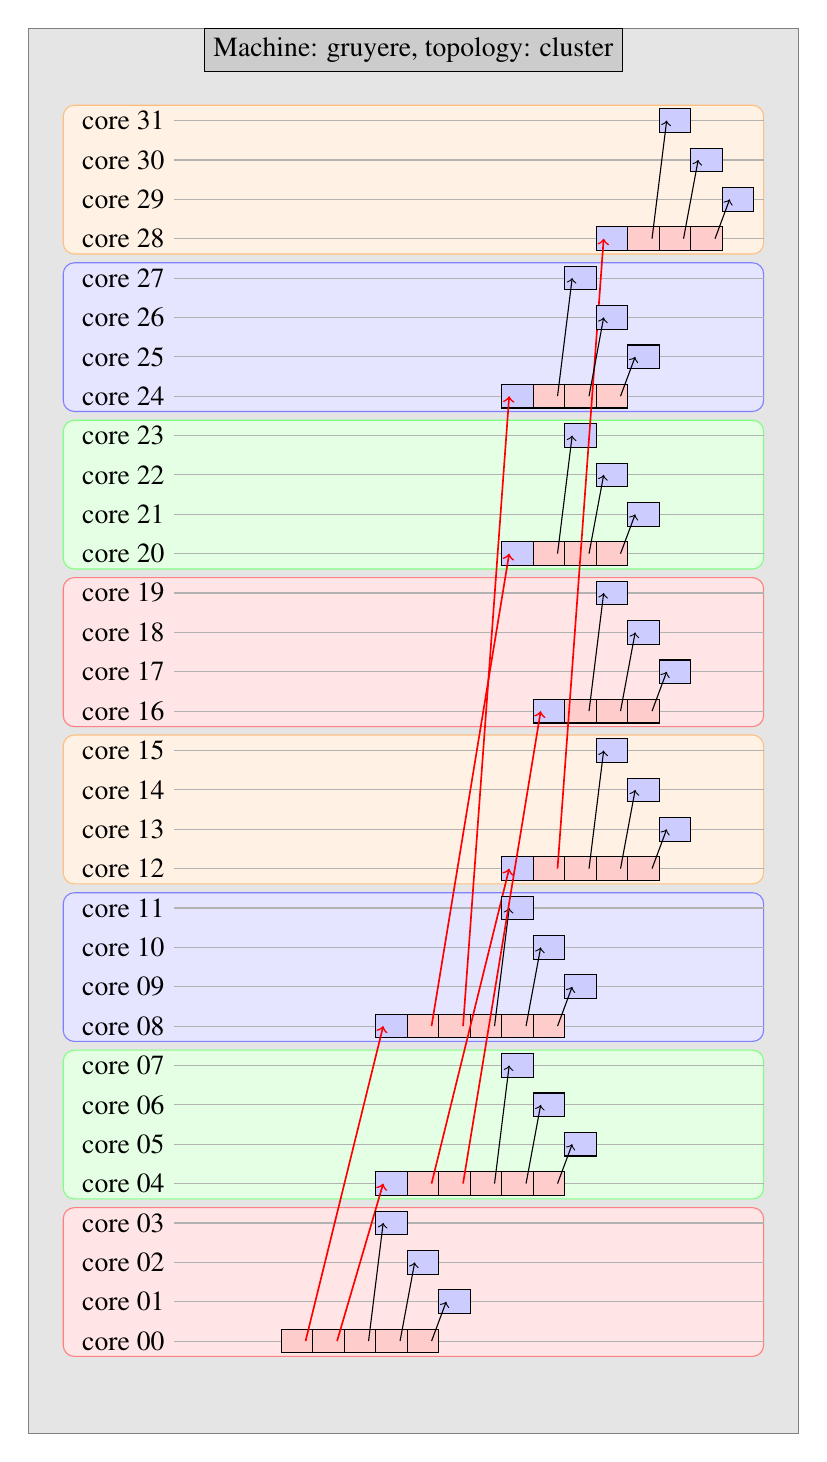
\begin{tikzpicture}[]
  % Insert visualization
  \node (core_0_label) at (0mm,0mm) {core 00};
\node (core_1_label) at (0mm,5mm) {core 01};
\node (core_2_label) at (0mm,10mm) {core 02};
\node (core_3_label) at (0mm,15mm) {core 03};
\node (core_4_label) at (0mm,20mm) {core 04};
\node (core_5_label) at (0mm,25mm) {core 05};
\node (core_6_label) at (0mm,30mm) {core 06};
\node (core_7_label) at (0mm,35mm) {core 07};
\node (core_8_label) at (0mm,40mm) {core 08};
\node (core_9_label) at (0mm,45mm) {core 09};
\node (core_10_label) at (0mm,50mm) {core 10};
\node (core_11_label) at (0mm,55mm) {core 11};
\node (core_12_label) at (0mm,60mm) {core 12};
\node (core_13_label) at (0mm,65mm) {core 13};
\node (core_14_label) at (0mm,70mm) {core 14};
\node (core_15_label) at (0mm,75mm) {core 15};
\node (core_16_label) at (0mm,80mm) {core 16};
\node (core_17_label) at (0mm,85mm) {core 17};
\node (core_18_label) at (0mm,90mm) {core 18};
\node (core_19_label) at (0mm,95mm) {core 19};
\node (core_20_label) at (0mm,100mm) {core 20};
\node (core_21_label) at (0mm,105mm) {core 21};
\node (core_22_label) at (0mm,110mm) {core 22};
\node (core_23_label) at (0mm,115mm) {core 23};
\node (core_24_label) at (0mm,120mm) {core 24};
\node (core_25_label) at (0mm,125mm) {core 25};
\node (core_26_label) at (0mm,130mm) {core 26};
\node (core_27_label) at (0mm,135mm) {core 27};
\node (core_28_label) at (0mm,140mm) {core 28};
\node (core_29_label) at (0mm,145mm) {core 29};
\node (core_30_label) at (0mm,150mm) {core 30};
\node (core_31_label) at (0mm,155mm) {core 31};
\node[draw,fill=red!20,minimum width=4mm, minimum height=3mm,anchor=west] (s_0_8) at (20mm,0mm) {};
\node[draw,fill=red!20,minimum width=4mm, minimum height=3mm,anchor=west] (s_0_4) at (24mm,0mm) {};
\node[draw,fill=red!20,minimum width=4mm, minimum height=3mm,anchor=west] (s_0_3) at (28mm,0mm) {};
\node[draw,fill=red!20,minimum width=4mm, minimum height=3mm,anchor=west] (s_0_2) at (32mm,0mm) {};
\node[draw,fill=red!20,minimum width=4mm, minimum height=3mm,anchor=west] (s_0_1) at (36mm,0mm) {};
\node[draw,fill=blue!20,minimum width=4mm, minimum height=3mm,anchor=west] (r_0_4) at (32mm,20mm) {};
\draw[->,semithick,color=red] ($(s_0_4.east)-(1mm,0mm)$) -- ($(r_0_4.west)+(1mm,0mm)$); 
\node[draw,fill=red!20,minimum width=4mm, minimum height=3mm,anchor=west] (s_4_12) at (36mm,20mm) {};
\node[draw,fill=red!20,minimum width=4mm, minimum height=3mm,anchor=west] (s_4_16) at (40mm,20mm) {};
\node[draw,fill=red!20,minimum width=4mm, minimum height=3mm,anchor=west] (s_4_7) at (44mm,20mm) {};
\node[draw,fill=red!20,minimum width=4mm, minimum height=3mm,anchor=west] (s_4_6) at (48mm,20mm) {};
\node[draw,fill=red!20,minimum width=4mm, minimum height=3mm,anchor=west] (s_4_5) at (52mm,20mm) {};
\node[draw,fill=blue!20,minimum width=4mm, minimum height=3mm,anchor=west] (r_0_8) at (32mm,40mm) {};
\draw[->,semithick,color=red] ($(s_0_8.east)-(1mm,0mm)$) -- ($(r_0_8.west)+(1mm,0mm)$); 
\node[draw,fill=red!20,minimum width=4mm, minimum height=3mm,anchor=west] (s_8_20) at (36mm,40mm) {};
\node[draw,fill=red!20,minimum width=4mm, minimum height=3mm,anchor=west] (s_8_24) at (40mm,40mm) {};
\node[draw,fill=red!20,minimum width=4mm, minimum height=3mm,anchor=west] (s_8_11) at (44mm,40mm) {};
\node[draw,fill=red!20,minimum width=4mm, minimum height=3mm,anchor=west] (s_8_10) at (48mm,40mm) {};
\node[draw,fill=red!20,minimum width=4mm, minimum height=3mm,anchor=west] (s_8_9) at (52mm,40mm) {};
\node[draw,fill=blue!20,minimum width=4mm, minimum height=3mm,anchor=west] (r_0_3) at (32mm,15mm) {};
\draw[->] ($(s_0_3.east)-(1mm,0mm)$) -- ($(r_0_3.west)+(1mm,0mm)$); 
\node[draw,fill=blue!20,minimum width=4mm, minimum height=3mm,anchor=west] (r_0_2) at (36mm,10mm) {};
\draw[->] ($(s_0_2.east)-(1mm,0mm)$) -- ($(r_0_2.west)+(1mm,0mm)$); 
\node[draw,fill=blue!20,minimum width=4mm, minimum height=3mm,anchor=west] (r_0_1) at (40mm,5mm) {};
\draw[->] ($(s_0_1.east)-(1mm,0mm)$) -- ($(r_0_1.west)+(1mm,0mm)$); 
\node[draw,fill=blue!20,minimum width=4mm, minimum height=3mm,anchor=west] (r_8_20) at (48mm,100mm) {};
\draw[->,semithick,color=red] ($(s_8_20.east)-(1mm,0mm)$) -- ($(r_8_20.west)+(1mm,0mm)$); 
\node[draw,fill=red!20,minimum width=4mm, minimum height=3mm,anchor=west] (s_20_23) at (52mm,100mm) {};
\node[draw,fill=red!20,minimum width=4mm, minimum height=3mm,anchor=west] (s_20_22) at (56mm,100mm) {};
\node[draw,fill=red!20,minimum width=4mm, minimum height=3mm,anchor=west] (s_20_21) at (60mm,100mm) {};
\node[draw,fill=blue!20,minimum width=4mm, minimum height=3mm,anchor=west] (r_8_24) at (48mm,120mm) {};
\draw[->,semithick,color=red] ($(s_8_24.east)-(1mm,0mm)$) -- ($(r_8_24.west)+(1mm,0mm)$); 
\node[draw,fill=red!20,minimum width=4mm, minimum height=3mm,anchor=west] (s_24_27) at (52mm,120mm) {};
\node[draw,fill=red!20,minimum width=4mm, minimum height=3mm,anchor=west] (s_24_26) at (56mm,120mm) {};
\node[draw,fill=red!20,minimum width=4mm, minimum height=3mm,anchor=west] (s_24_25) at (60mm,120mm) {};
\node[draw,fill=blue!20,minimum width=4mm, minimum height=3mm,anchor=west] (r_4_12) at (48mm,60mm) {};
\draw[->,semithick,color=red] ($(s_4_12.east)-(1mm,0mm)$) -- ($(r_4_12.west)+(1mm,0mm)$); 
\node[draw,fill=red!20,minimum width=4mm, minimum height=3mm,anchor=west] (s_12_28) at (52mm,60mm) {};
\node[draw,fill=red!20,minimum width=4mm, minimum height=3mm,anchor=west] (s_12_15) at (56mm,60mm) {};
\node[draw,fill=red!20,minimum width=4mm, minimum height=3mm,anchor=west] (s_12_14) at (60mm,60mm) {};
\node[draw,fill=red!20,minimum width=4mm, minimum height=3mm,anchor=west] (s_12_13) at (64mm,60mm) {};
\node[draw,fill=blue!20,minimum width=4mm, minimum height=3mm,anchor=west] (r_8_11) at (48mm,55mm) {};
\draw[->] ($(s_8_11.east)-(1mm,0mm)$) -- ($(r_8_11.west)+(1mm,0mm)$); 
\node[draw,fill=blue!20,minimum width=4mm, minimum height=3mm,anchor=west] (r_4_7) at (48mm,35mm) {};
\draw[->] ($(s_4_7.east)-(1mm,0mm)$) -- ($(r_4_7.west)+(1mm,0mm)$); 
\node[draw,fill=blue!20,minimum width=4mm, minimum height=3mm,anchor=west] (r_4_16) at (52mm,80mm) {};
\draw[->,semithick,color=red] ($(s_4_16.east)-(1mm,0mm)$) -- ($(r_4_16.west)+(1mm,0mm)$); 
\node[draw,fill=red!20,minimum width=4mm, minimum height=3mm,anchor=west] (s_16_19) at (56mm,80mm) {};
\node[draw,fill=red!20,minimum width=4mm, minimum height=3mm,anchor=west] (s_16_18) at (60mm,80mm) {};
\node[draw,fill=red!20,minimum width=4mm, minimum height=3mm,anchor=west] (s_16_17) at (64mm,80mm) {};
\node[draw,fill=blue!20,minimum width=4mm, minimum height=3mm,anchor=west] (r_8_10) at (52mm,50mm) {};
\draw[->] ($(s_8_10.east)-(1mm,0mm)$) -- ($(r_8_10.west)+(1mm,0mm)$); 
\node[draw,fill=blue!20,minimum width=4mm, minimum height=3mm,anchor=west] (r_4_6) at (52mm,30mm) {};
\draw[->] ($(s_4_6.east)-(1mm,0mm)$) -- ($(r_4_6.west)+(1mm,0mm)$); 
\node[draw,fill=blue!20,minimum width=4mm, minimum height=3mm,anchor=west] (r_20_23) at (56mm,115mm) {};
\draw[->] ($(s_20_23.east)-(1mm,0mm)$) -- ($(r_20_23.west)+(1mm,0mm)$); 
\node[draw,fill=blue!20,minimum width=4mm, minimum height=3mm,anchor=west] (r_24_27) at (56mm,135mm) {};
\draw[->] ($(s_24_27.east)-(1mm,0mm)$) -- ($(r_24_27.west)+(1mm,0mm)$); 
\node[draw,fill=blue!20,minimum width=4mm, minimum height=3mm,anchor=west] (r_8_9) at (56mm,45mm) {};
\draw[->] ($(s_8_9.east)-(1mm,0mm)$) -- ($(r_8_9.west)+(1mm,0mm)$); 
\node[draw,fill=blue!20,minimum width=4mm, minimum height=3mm,anchor=west] (r_4_5) at (56mm,25mm) {};
\draw[->] ($(s_4_5.east)-(1mm,0mm)$) -- ($(r_4_5.west)+(1mm,0mm)$); 
\node[draw,fill=blue!20,minimum width=4mm, minimum height=3mm,anchor=west] (r_12_28) at (60mm,140mm) {};
\draw[->,semithick,color=red] ($(s_12_28.east)-(1mm,0mm)$) -- ($(r_12_28.west)+(1mm,0mm)$); 
\node[draw,fill=red!20,minimum width=4mm, minimum height=3mm,anchor=west] (s_28_31) at (64mm,140mm) {};
\node[draw,fill=red!20,minimum width=4mm, minimum height=3mm,anchor=west] (s_28_30) at (68mm,140mm) {};
\node[draw,fill=red!20,minimum width=4mm, minimum height=3mm,anchor=west] (s_28_29) at (72mm,140mm) {};
\node[draw,fill=blue!20,minimum width=4mm, minimum height=3mm,anchor=west] (r_24_26) at (60mm,130mm) {};
\draw[->] ($(s_24_26.east)-(1mm,0mm)$) -- ($(r_24_26.west)+(1mm,0mm)$); 
\node[draw,fill=blue!20,minimum width=4mm, minimum height=3mm,anchor=west] (r_20_22) at (60mm,110mm) {};
\draw[->] ($(s_20_22.east)-(1mm,0mm)$) -- ($(r_20_22.west)+(1mm,0mm)$); 
\node[draw,fill=blue!20,minimum width=4mm, minimum height=3mm,anchor=west] (r_12_15) at (60mm,75mm) {};
\draw[->] ($(s_12_15.east)-(1mm,0mm)$) -- ($(r_12_15.west)+(1mm,0mm)$); 
\node[draw,fill=blue!20,minimum width=4mm, minimum height=3mm,anchor=west] (r_16_19) at (60mm,95mm) {};
\draw[->] ($(s_16_19.east)-(1mm,0mm)$) -- ($(r_16_19.west)+(1mm,0mm)$); 
\node[draw,fill=blue!20,minimum width=4mm, minimum height=3mm,anchor=west] (r_24_25) at (64mm,125mm) {};
\draw[->] ($(s_24_25.east)-(1mm,0mm)$) -- ($(r_24_25.west)+(1mm,0mm)$); 
\node[draw,fill=blue!20,minimum width=4mm, minimum height=3mm,anchor=west] (r_12_14) at (64mm,70mm) {};
\draw[->] ($(s_12_14.east)-(1mm,0mm)$) -- ($(r_12_14.west)+(1mm,0mm)$); 
\node[draw,fill=blue!20,minimum width=4mm, minimum height=3mm,anchor=west] (r_20_21) at (64mm,105mm) {};
\draw[->] ($(s_20_21.east)-(1mm,0mm)$) -- ($(r_20_21.west)+(1mm,0mm)$); 
\node[draw,fill=blue!20,minimum width=4mm, minimum height=3mm,anchor=west] (r_16_18) at (64mm,90mm) {};
\draw[->] ($(s_16_18.east)-(1mm,0mm)$) -- ($(r_16_18.west)+(1mm,0mm)$); 
\node[draw,fill=blue!20,minimum width=4mm, minimum height=3mm,anchor=west] (r_16_17) at (68mm,85mm) {};
\draw[->] ($(s_16_17.east)-(1mm,0mm)$) -- ($(r_16_17.west)+(1mm,0mm)$); 
\node[draw,fill=blue!20,minimum width=4mm, minimum height=3mm,anchor=west] (r_12_13) at (68mm,65mm) {};
\draw[->] ($(s_12_13.east)-(1mm,0mm)$) -- ($(r_12_13.west)+(1mm,0mm)$); 
\node[draw,fill=blue!20,minimum width=4mm, minimum height=3mm,anchor=west] (r_28_31) at (68mm,155mm) {};
\draw[->] ($(s_28_31.east)-(1mm,0mm)$) -- ($(r_28_31.west)+(1mm,0mm)$); 
\node[draw,fill=blue!20,minimum width=4mm, minimum height=3mm,anchor=west] (r_28_30) at (72mm,150mm) {};
\draw[->] ($(s_28_30.east)-(1mm,0mm)$) -- ($(r_28_30.west)+(1mm,0mm)$); 
\node[draw,fill=blue!20,minimum width=4mm, minimum height=3mm,anchor=west] (r_28_29) at (76mm,145mm) {};
\draw[->] ($(s_28_29.east)-(1mm,0mm)$) -- ($(r_28_29.west)+(1mm,0mm)$); 
\begin{pgfonlayer}{background}
\node [fit=(core_0_label) (core_1_label) (core_2_label) (core_3_label) (core_4_label) (core_5_label) (core_6_label) (core_7_label) (core_8_label) (core_9_label) (core_10_label) (core_11_label) (core_12_label) (core_13_label) (core_14_label) (core_15_label) (core_16_label) (core_17_label) (core_18_label) (core_19_label) (core_20_label) (core_21_label) (core_22_label) (core_23_label) (core_24_label) (core_25_label) (core_26_label) (core_27_label) (core_28_label) (core_29_label) (core_30_label) (core_31_label) (s_0_8) (s_0_4) (s_0_3) (s_0_2) (s_0_1) (r_0_4) (s_4_12) (s_4_16) (s_4_7) (s_4_6) (s_4_5) (r_0_8) (s_8_20) (s_8_24) (s_8_11) (s_8_10) (s_8_9) (r_0_3) (r_0_2) (r_0_1) (r_4_12) (s_12_28) (s_12_15) (s_12_14) (s_12_13) (r_8_24) (s_24_27) (s_24_26) (s_24_25) (r_8_20) (s_20_23) (s_20_22) (s_20_21) (r_4_7) (r_8_11) (r_4_16) (s_16_19) (s_16_18) (s_16_17) (r_8_10) (r_4_6) (r_4_5) (r_20_23) (r_8_9) (r_24_27) (r_12_28) (s_28_31) (s_28_30) (s_28_29) (r_24_26) (r_16_19) (r_12_15) (r_20_22) (r_12_14) (r_20_21) (r_24_25) (r_16_18) (r_28_31) (r_12_13) (r_16_17) (r_28_30) (r_28_29) (core_0_label) (core_1_label) (core_2_label) (core_3_label) (core_4_label) (core_5_label) (core_6_label) (core_7_label) (core_8_label) (core_9_label) (core_10_label) (core_11_label) (core_12_label) (core_13_label) (core_14_label) (core_15_label) (core_16_label) (core_17_label) (core_18_label) (core_19_label) (core_20_label) (core_21_label) (core_22_label) (core_23_label) (core_24_label) (core_25_label) (core_26_label) (core_27_label) (core_28_label) (core_29_label) (core_30_label) (core_31_label) (s_0_8) (s_0_4) (s_0_3) (s_0_2) (s_0_1) (r_0_4) (s_4_12) (s_4_16) (s_4_7) (s_4_6) (s_4_5) (r_0_8) (s_8_20) (s_8_24) (s_8_11) (s_8_10) (s_8_9) (r_0_3) (r_0_2) (r_0_1) (r_8_20) (s_20_23) (s_20_22) (s_20_21) (r_8_24) (s_24_27) (s_24_26) (s_24_25) (r_4_12) (s_12_28) (s_12_15) (s_12_14) (s_12_13) (r_8_11) (r_4_7) (r_4_16) (s_16_19) (s_16_18) (s_16_17) (r_8_10) (r_4_6) (r_20_23) (r_24_27) (r_8_9) (r_4_5) (r_12_28) (s_28_31) (s_28_30) (s_28_29) (r_24_26) (r_20_22) (r_12_15) (r_16_19) (r_24_25) (r_12_14) (r_20_21) (r_16_18) (r_16_17) (r_12_13) (r_28_31) (r_28_30) (r_28_29)] (allobjects) {};
\node [draw=black!50,fill=black!10,fit=(core_0_label) (core_1_label) (core_2_label) (core_3_label) (core_4_label) (core_5_label) (core_6_label) (core_7_label) (core_8_label) (core_9_label) (core_10_label) (core_11_label) (core_12_label) (core_13_label) (core_14_label) (core_15_label) (core_16_label) (core_17_label) (core_18_label) (core_19_label) (core_20_label) (core_21_label) (core_22_label) (core_23_label) (core_24_label) (core_25_label) (core_26_label) (core_27_label) (core_28_label) (core_29_label) (core_30_label) (core_31_label) (s_0_8) (s_0_4) (s_0_3) (s_0_2) (s_0_1) (r_0_4) (s_4_12) (s_4_16) (s_4_7) (s_4_6) (s_4_5) (r_0_8) (s_8_20) (s_8_24) (s_8_11) (s_8_10) (s_8_9) (r_0_3) (r_0_2) (r_0_1) (r_4_12) (s_12_28) (s_12_15) (s_12_14) (s_12_13) (r_8_24) (s_24_27) (s_24_26) (s_24_25) (r_8_20) (s_20_23) (s_20_22) (s_20_21) (r_4_7) (r_8_11) (r_4_16) (s_16_19) (s_16_18) (s_16_17) (r_8_10) (r_4_6) (r_4_5) (r_20_23) (r_8_9) (r_24_27) (r_12_28) (s_28_31) (s_28_30) (s_28_29) (r_24_26) (r_16_19) (r_12_15) (r_20_22) (r_12_14) (r_20_21) (r_24_25) (r_16_18) (r_28_31) (r_12_13) (r_16_17) (r_28_30) (r_28_29) (core_0_label) (core_1_label) (core_2_label) (core_3_label) (core_4_label) (core_5_label) (core_6_label) (core_7_label) (core_8_label) (core_9_label) (core_10_label) (core_11_label) (core_12_label) (core_13_label) (core_14_label) (core_15_label) (core_16_label) (core_17_label) (core_18_label) (core_19_label) (core_20_label) (core_21_label) (core_22_label) (core_23_label) (core_24_label) (core_25_label) (core_26_label) (core_27_label) (core_28_label) (core_29_label) (core_30_label) (core_31_label) (s_0_8) (s_0_4) (s_0_3) (s_0_2) (s_0_1) (r_0_4) (s_4_12) (s_4_16) (s_4_7) (s_4_6) (s_4_5) (r_0_8) (s_8_20) (s_8_24) (s_8_11) (s_8_10) (s_8_9) (r_0_3) (r_0_2) (r_0_1) (r_8_20) (s_20_23) (s_20_22) (s_20_21) (r_8_24) (s_24_27) (s_24_26) (s_24_25) (r_4_12) (s_12_28) (s_12_15) (s_12_14) (s_12_13) (r_8_11) (r_4_7) (r_4_16) (s_16_19) (s_16_18) (s_16_17) (r_8_10) (r_4_6) (r_20_23) (r_24_27) (r_8_9) (r_4_5) (r_12_28) (s_28_31) (s_28_30) (s_28_29) (r_24_26) (r_20_22) (r_12_15) (r_16_19) (r_24_25) (r_12_14) (r_20_21) (r_16_18) (r_16_17) (r_12_13) (r_28_31) (r_28_30) (r_28_29),scale=1.1] (bg) {};
\draw let \p1 = (allobjects.east) in node[] (numa_axis_0) at (\x1,0mm) {};
\draw let \p1 = (allobjects.east) in node[] (numa_axis_1) at (\x1,5mm) {};
\draw let \p1 = (allobjects.east) in node[] (numa_axis_2) at (\x1,10mm) {};
\draw let \p1 = (allobjects.east) in node[] (numa_axis_3) at (\x1,15mm) {};
\draw let \p1 = (allobjects.east) in node[] (numa_axis_4) at (\x1,20mm) {};
\draw let \p1 = (allobjects.east) in node[] (numa_axis_5) at (\x1,25mm) {};
\draw let \p1 = (allobjects.east) in node[] (numa_axis_6) at (\x1,30mm) {};
\draw let \p1 = (allobjects.east) in node[] (numa_axis_7) at (\x1,35mm) {};
\draw let \p1 = (allobjects.east) in node[] (numa_axis_8) at (\x1,40mm) {};
\draw let \p1 = (allobjects.east) in node[] (numa_axis_9) at (\x1,45mm) {};
\draw let \p1 = (allobjects.east) in node[] (numa_axis_10) at (\x1,50mm) {};
\draw let \p1 = (allobjects.east) in node[] (numa_axis_11) at (\x1,55mm) {};
\draw let \p1 = (allobjects.east) in node[] (numa_axis_12) at (\x1,60mm) {};
\draw let \p1 = (allobjects.east) in node[] (numa_axis_13) at (\x1,65mm) {};
\draw let \p1 = (allobjects.east) in node[] (numa_axis_14) at (\x1,70mm) {};
\draw let \p1 = (allobjects.east) in node[] (numa_axis_15) at (\x1,75mm) {};
\draw let \p1 = (allobjects.east) in node[] (numa_axis_16) at (\x1,80mm) {};
\draw let \p1 = (allobjects.east) in node[] (numa_axis_17) at (\x1,85mm) {};
\draw let \p1 = (allobjects.east) in node[] (numa_axis_18) at (\x1,90mm) {};
\draw let \p1 = (allobjects.east) in node[] (numa_axis_19) at (\x1,95mm) {};
\draw let \p1 = (allobjects.east) in node[] (numa_axis_20) at (\x1,100mm) {};
\draw let \p1 = (allobjects.east) in node[] (numa_axis_21) at (\x1,105mm) {};
\draw let \p1 = (allobjects.east) in node[] (numa_axis_22) at (\x1,110mm) {};
\draw let \p1 = (allobjects.east) in node[] (numa_axis_23) at (\x1,115mm) {};
\draw let \p1 = (allobjects.east) in node[] (numa_axis_24) at (\x1,120mm) {};
\draw let \p1 = (allobjects.east) in node[] (numa_axis_25) at (\x1,125mm) {};
\draw let \p1 = (allobjects.east) in node[] (numa_axis_26) at (\x1,130mm) {};
\draw let \p1 = (allobjects.east) in node[] (numa_axis_27) at (\x1,135mm) {};
\draw let \p1 = (allobjects.east) in node[] (numa_axis_28) at (\x1,140mm) {};
\draw let \p1 = (allobjects.east) in node[] (numa_axis_29) at (\x1,145mm) {};
\draw let \p1 = (allobjects.east) in node[] (numa_axis_30) at (\x1,150mm) {};
\draw let \p1 = (allobjects.east) in node[] (numa_axis_31) at (\x1,155mm) {};
\node [yscale=0.85,draw=red!50,fill=red!10,fit=(core_0_label) (core_1_label) (core_2_label) (core_3_label) (s_0_8) (s_0_4) (s_0_3) (s_0_2) (s_0_1) (r_0_3) (r_0_2) (r_0_1) (numa_axis_0.west) (core_0_label) (core_1_label) (core_2_label) (core_3_label) (s_0_8) (s_0_4) (s_0_3) (s_0_2) (s_0_1) (r_0_3) (r_0_2) (r_0_1) (numa_axis_0.west),rounded corners] {};
\node [yscale=0.85,draw=green!50,fill=green!10,fit=(core_4_label) (core_5_label) (core_6_label) (core_7_label) (r_0_4) (s_4_12) (s_4_16) (s_4_7) (s_4_6) (s_4_5) (r_4_7) (r_4_6) (r_4_5) (numa_axis_4.west) (core_4_label) (core_5_label) (core_6_label) (core_7_label) (r_0_4) (s_4_12) (s_4_16) (s_4_7) (s_4_6) (s_4_5) (r_4_7) (r_4_6) (r_4_5) (numa_axis_4.west),rounded corners] {};
\node [yscale=0.85,draw=blue!50,fill=blue!10,fit=(core_8_label) (core_9_label) (core_10_label) (core_11_label) (r_0_8) (s_8_20) (s_8_24) (s_8_11) (s_8_10) (s_8_9) (r_8_11) (r_8_10) (r_8_9) (numa_axis_8.west) (core_8_label) (core_9_label) (core_10_label) (core_11_label) (r_0_8) (s_8_20) (s_8_24) (s_8_11) (s_8_10) (s_8_9) (r_8_11) (r_8_10) (r_8_9) (numa_axis_8.west),rounded corners] {};
\node [yscale=0.85,draw=orange!50,fill=orange!10,fit=(core_12_label) (core_13_label) (core_14_label) (core_15_label) (r_4_12) (s_12_28) (s_12_15) (s_12_14) (s_12_13) (r_12_15) (r_12_14) (r_12_13) (numa_axis_12.west) (core_12_label) (core_13_label) (core_14_label) (core_15_label) (r_4_12) (s_12_28) (s_12_15) (s_12_14) (s_12_13) (r_12_15) (r_12_14) (r_12_13) (numa_axis_12.west),rounded corners] {};
\node [yscale=0.85,draw=red!50,fill=red!10,fit=(core_16_label) (core_17_label) (core_18_label) (core_19_label) (r_4_16) (s_16_19) (s_16_18) (s_16_17) (r_16_19) (r_16_18) (r_16_17) (numa_axis_16.west) (core_16_label) (core_17_label) (core_18_label) (core_19_label) (r_4_16) (s_16_19) (s_16_18) (s_16_17) (r_16_19) (r_16_18) (r_16_17) (numa_axis_16.west),rounded corners] {};
\node [yscale=0.85,draw=green!50,fill=green!10,fit=(core_20_label) (core_21_label) (core_22_label) (core_23_label) (r_8_20) (s_20_23) (s_20_22) (s_20_21) (r_20_23) (r_20_22) (r_20_21) (numa_axis_20.west) (core_20_label) (core_21_label) (core_22_label) (core_23_label) (r_8_20) (s_20_23) (s_20_22) (s_20_21) (r_20_23) (r_20_22) (r_20_21) (numa_axis_20.west),rounded corners] {};
\node [yscale=0.85,draw=blue!50,fill=blue!10,fit=(core_24_label) (core_25_label) (core_26_label) (core_27_label) (r_8_24) (s_24_27) (s_24_26) (s_24_25) (r_24_27) (r_24_26) (r_24_25) (numa_axis_24.west) (core_24_label) (core_25_label) (core_26_label) (core_27_label) (r_8_24) (s_24_27) (s_24_26) (s_24_25) (r_24_27) (r_24_26) (r_24_25) (numa_axis_24.west),rounded corners] {};
\node [yscale=0.85,draw=orange!50,fill=orange!10,fit=(core_28_label) (core_29_label) (core_30_label) (core_31_label) (r_12_28) (s_28_31) (s_28_30) (s_28_29) (r_28_31) (r_28_30) (r_28_29) (numa_axis_28.west) (core_28_label) (core_29_label) (core_30_label) (core_31_label) (r_12_28) (s_28_31) (s_28_30) (s_28_29) (r_28_31) (r_28_30) (r_28_29) (numa_axis_28.west),rounded corners] {};
\draw[color=black!30] let \p1 = (core_10_label.east), \p2 = (allobjects.east) in (\x1,0mm) -- (\x2,0mm);
\draw[color=black!30] let \p1 = (core_10_label.east), \p2 = (allobjects.east) in (\x1,5mm) -- (\x2,5mm);
\draw[color=black!30] let \p1 = (core_10_label.east), \p2 = (allobjects.east) in (\x1,10mm) -- (\x2,10mm);
\draw[color=black!30] let \p1 = (core_10_label.east), \p2 = (allobjects.east) in (\x1,15mm) -- (\x2,15mm);
\draw[color=black!30] let \p1 = (core_10_label.east), \p2 = (allobjects.east) in (\x1,20mm) -- (\x2,20mm);
\draw[color=black!30] let \p1 = (core_10_label.east), \p2 = (allobjects.east) in (\x1,25mm) -- (\x2,25mm);
\draw[color=black!30] let \p1 = (core_10_label.east), \p2 = (allobjects.east) in (\x1,30mm) -- (\x2,30mm);
\draw[color=black!30] let \p1 = (core_10_label.east), \p2 = (allobjects.east) in (\x1,35mm) -- (\x2,35mm);
\draw[color=black!30] let \p1 = (core_10_label.east), \p2 = (allobjects.east) in (\x1,40mm) -- (\x2,40mm);
\draw[color=black!30] let \p1 = (core_10_label.east), \p2 = (allobjects.east) in (\x1,45mm) -- (\x2,45mm);
\draw[color=black!30] let \p1 = (core_10_label.east), \p2 = (allobjects.east) in (\x1,50mm) -- (\x2,50mm);
\draw[color=black!30] let \p1 = (core_10_label.east), \p2 = (allobjects.east) in (\x1,55mm) -- (\x2,55mm);
\draw[color=black!30] let \p1 = (core_10_label.east), \p2 = (allobjects.east) in (\x1,60mm) -- (\x2,60mm);
\draw[color=black!30] let \p1 = (core_10_label.east), \p2 = (allobjects.east) in (\x1,65mm) -- (\x2,65mm);
\draw[color=black!30] let \p1 = (core_10_label.east), \p2 = (allobjects.east) in (\x1,70mm) -- (\x2,70mm);
\draw[color=black!30] let \p1 = (core_10_label.east), \p2 = (allobjects.east) in (\x1,75mm) -- (\x2,75mm);
\draw[color=black!30] let \p1 = (core_10_label.east), \p2 = (allobjects.east) in (\x1,80mm) -- (\x2,80mm);
\draw[color=black!30] let \p1 = (core_10_label.east), \p2 = (allobjects.east) in (\x1,85mm) -- (\x2,85mm);
\draw[color=black!30] let \p1 = (core_10_label.east), \p2 = (allobjects.east) in (\x1,90mm) -- (\x2,90mm);
\draw[color=black!30] let \p1 = (core_10_label.east), \p2 = (allobjects.east) in (\x1,95mm) -- (\x2,95mm);
\draw[color=black!30] let \p1 = (core_10_label.east), \p2 = (allobjects.east) in (\x1,100mm) -- (\x2,100mm);
\draw[color=black!30] let \p1 = (core_10_label.east), \p2 = (allobjects.east) in (\x1,105mm) -- (\x2,105mm);
\draw[color=black!30] let \p1 = (core_10_label.east), \p2 = (allobjects.east) in (\x1,110mm) -- (\x2,110mm);
\draw[color=black!30] let \p1 = (core_10_label.east), \p2 = (allobjects.east) in (\x1,115mm) -- (\x2,115mm);
\draw[color=black!30] let \p1 = (core_10_label.east), \p2 = (allobjects.east) in (\x1,120mm) -- (\x2,120mm);
\draw[color=black!30] let \p1 = (core_10_label.east), \p2 = (allobjects.east) in (\x1,125mm) -- (\x2,125mm);
\draw[color=black!30] let \p1 = (core_10_label.east), \p2 = (allobjects.east) in (\x1,130mm) -- (\x2,130mm);
\draw[color=black!30] let \p1 = (core_10_label.east), \p2 = (allobjects.east) in (\x1,135mm) -- (\x2,135mm);
\draw[color=black!30] let \p1 = (core_10_label.east), \p2 = (allobjects.east) in (\x1,140mm) -- (\x2,140mm);
\draw[color=black!30] let \p1 = (core_10_label.east), \p2 = (allobjects.east) in (\x1,145mm) -- (\x2,145mm);
\draw[color=black!30] let \p1 = (core_10_label.east), \p2 = (allobjects.east) in (\x1,150mm) -- (\x2,150mm);
\draw[color=black!30] let \p1 = (core_10_label.east), \p2 = (allobjects.east) in (\x1,155mm) -- (\x2,155mm);
\node[draw=black,anchor=north,fill=black!20] at (bg.north) {Machine: gruyere, topology: cluster};
\end{pgfonlayer}

\end{tikzpicture}
\newpage
\subsubsection{mst}
\begin{tikzpicture}[]
  % Insert visualization
  \input{graphs/visu_gruyere_mst}
\end{tikzpicture}
\newpage
\subsubsection{bintree}
\begin{tikzpicture}[]
  % Insert visualization
  \input{graphs/visu_gruyere_bintree}
\end{tikzpicture}
\newpage
\subsubsection{sequential}
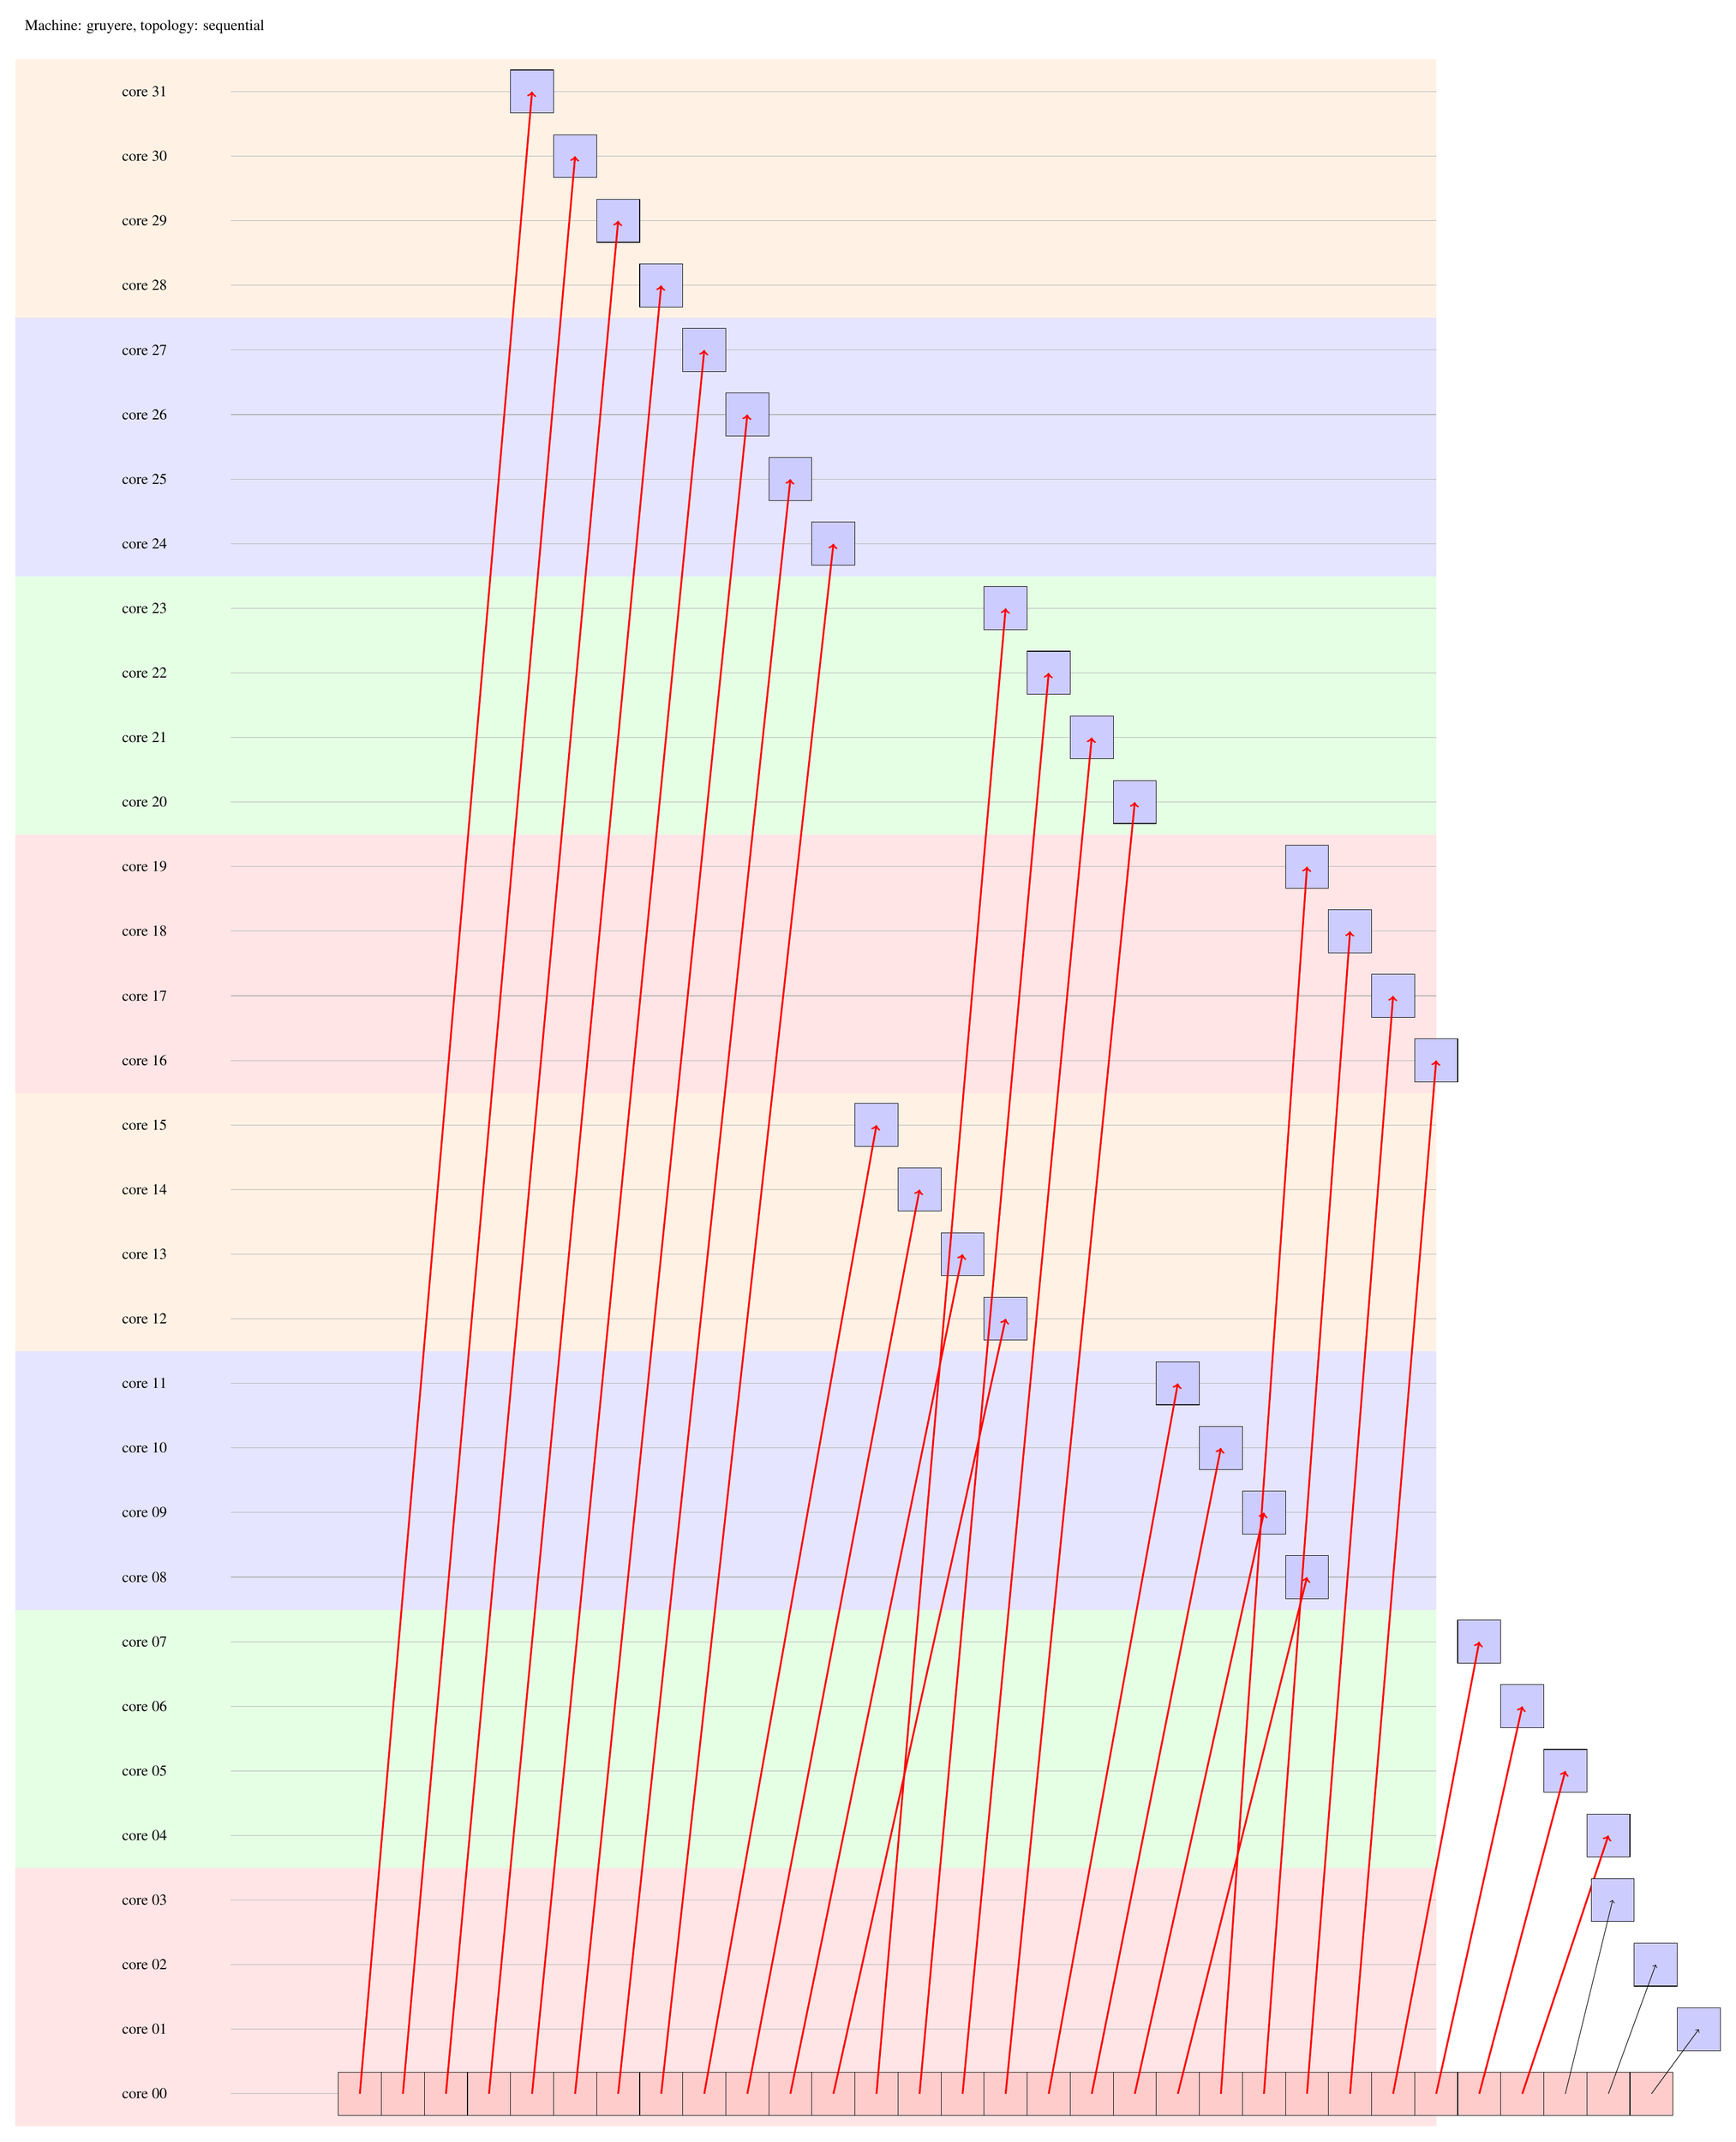
\begin{tikzpicture}[]
  % Insert visualization
  \draw[fill,color=red!10] (-3cm,7.500000mm) rectangle (30cm,-7.500000mm);
\node at (0mm,0mm) {core 00};
\draw[color=black!30] (20mm,0mm) -- (30cm,0mm);
\draw[fill,color=red!10] (-3cm,22.500000mm) rectangle (30cm,7.500000mm);
\node at (0mm,15mm) {core 01};
\draw[color=black!30] (20mm,15mm) -- (30cm,15mm);
\draw[fill,color=red!10] (-3cm,37.500000mm) rectangle (30cm,22.500000mm);
\node at (0mm,30mm) {core 02};
\draw[color=black!30] (20mm,30mm) -- (30cm,30mm);
\draw[fill,color=red!10] (-3cm,52.500000mm) rectangle (30cm,37.500000mm);
\node at (0mm,45mm) {core 03};
\draw[color=black!30] (20mm,45mm) -- (30cm,45mm);
\draw[fill,color=green!10] (-3cm,67.500000mm) rectangle (30cm,52.500000mm);
\node at (0mm,60mm) {core 04};
\draw[color=black!30] (20mm,60mm) -- (30cm,60mm);
\draw[fill,color=green!10] (-3cm,82.500000mm) rectangle (30cm,67.500000mm);
\node at (0mm,75mm) {core 05};
\draw[color=black!30] (20mm,75mm) -- (30cm,75mm);
\draw[fill,color=green!10] (-3cm,97.500000mm) rectangle (30cm,82.500000mm);
\node at (0mm,90mm) {core 06};
\draw[color=black!30] (20mm,90mm) -- (30cm,90mm);
\draw[fill,color=green!10] (-3cm,112.500000mm) rectangle (30cm,97.500000mm);
\node at (0mm,105mm) {core 07};
\draw[color=black!30] (20mm,105mm) -- (30cm,105mm);
\draw[fill,color=blue!10] (-3cm,127.500000mm) rectangle (30cm,112.500000mm);
\node at (0mm,120mm) {core 08};
\draw[color=black!30] (20mm,120mm) -- (30cm,120mm);
\draw[fill,color=blue!10] (-3cm,142.500000mm) rectangle (30cm,127.500000mm);
\node at (0mm,135mm) {core 09};
\draw[color=black!30] (20mm,135mm) -- (30cm,135mm);
\draw[fill,color=blue!10] (-3cm,157.500000mm) rectangle (30cm,142.500000mm);
\node at (0mm,150mm) {core 10};
\draw[color=black!30] (20mm,150mm) -- (30cm,150mm);
\draw[fill,color=blue!10] (-3cm,172.500000mm) rectangle (30cm,157.500000mm);
\node at (0mm,165mm) {core 11};
\draw[color=black!30] (20mm,165mm) -- (30cm,165mm);
\draw[fill,color=orange!10] (-3cm,187.500000mm) rectangle (30cm,172.500000mm);
\node at (0mm,180mm) {core 12};
\draw[color=black!30] (20mm,180mm) -- (30cm,180mm);
\draw[fill,color=orange!10] (-3cm,202.500000mm) rectangle (30cm,187.500000mm);
\node at (0mm,195mm) {core 13};
\draw[color=black!30] (20mm,195mm) -- (30cm,195mm);
\draw[fill,color=orange!10] (-3cm,217.500000mm) rectangle (30cm,202.500000mm);
\node at (0mm,210mm) {core 14};
\draw[color=black!30] (20mm,210mm) -- (30cm,210mm);
\draw[fill,color=orange!10] (-3cm,232.500000mm) rectangle (30cm,217.500000mm);
\node at (0mm,225mm) {core 15};
\draw[color=black!30] (20mm,225mm) -- (30cm,225mm);
\draw[fill,color=red!10] (-3cm,247.500000mm) rectangle (30cm,232.500000mm);
\node at (0mm,240mm) {core 16};
\draw[color=black!30] (20mm,240mm) -- (30cm,240mm);
\draw[fill,color=red!10] (-3cm,262.500000mm) rectangle (30cm,247.500000mm);
\node at (0mm,255mm) {core 17};
\draw[color=black!30] (20mm,255mm) -- (30cm,255mm);
\draw[fill,color=red!10] (-3cm,277.500000mm) rectangle (30cm,262.500000mm);
\node at (0mm,270mm) {core 18};
\draw[color=black!30] (20mm,270mm) -- (30cm,270mm);
\draw[fill,color=red!10] (-3cm,292.500000mm) rectangle (30cm,277.500000mm);
\node at (0mm,285mm) {core 19};
\draw[color=black!30] (20mm,285mm) -- (30cm,285mm);
\draw[fill,color=green!10] (-3cm,307.500000mm) rectangle (30cm,292.500000mm);
\node at (0mm,300mm) {core 20};
\draw[color=black!30] (20mm,300mm) -- (30cm,300mm);
\draw[fill,color=green!10] (-3cm,322.500000mm) rectangle (30cm,307.500000mm);
\node at (0mm,315mm) {core 21};
\draw[color=black!30] (20mm,315mm) -- (30cm,315mm);
\draw[fill,color=green!10] (-3cm,337.500000mm) rectangle (30cm,322.500000mm);
\node at (0mm,330mm) {core 22};
\draw[color=black!30] (20mm,330mm) -- (30cm,330mm);
\draw[fill,color=green!10] (-3cm,352.500000mm) rectangle (30cm,337.500000mm);
\node at (0mm,345mm) {core 23};
\draw[color=black!30] (20mm,345mm) -- (30cm,345mm);
\draw[fill,color=blue!10] (-3cm,367.500000mm) rectangle (30cm,352.500000mm);
\node at (0mm,360mm) {core 24};
\draw[color=black!30] (20mm,360mm) -- (30cm,360mm);
\draw[fill,color=blue!10] (-3cm,382.500000mm) rectangle (30cm,367.500000mm);
\node at (0mm,375mm) {core 25};
\draw[color=black!30] (20mm,375mm) -- (30cm,375mm);
\draw[fill,color=blue!10] (-3cm,397.500000mm) rectangle (30cm,382.500000mm);
\node at (0mm,390mm) {core 26};
\draw[color=black!30] (20mm,390mm) -- (30cm,390mm);
\draw[fill,color=blue!10] (-3cm,412.500000mm) rectangle (30cm,397.500000mm);
\node at (0mm,405mm) {core 27};
\draw[color=black!30] (20mm,405mm) -- (30cm,405mm);
\draw[fill,color=orange!10] (-3cm,427.500000mm) rectangle (30cm,412.500000mm);
\node at (0mm,420mm) {core 28};
\draw[color=black!30] (20mm,420mm) -- (30cm,420mm);
\draw[fill,color=orange!10] (-3cm,442.500000mm) rectangle (30cm,427.500000mm);
\node at (0mm,435mm) {core 29};
\draw[color=black!30] (20mm,435mm) -- (30cm,435mm);
\draw[fill,color=orange!10] (-3cm,457.500000mm) rectangle (30cm,442.500000mm);
\node at (0mm,450mm) {core 30};
\draw[color=black!30] (20mm,450mm) -- (30cm,450mm);
\draw[fill,color=orange!10] (-3cm,472.500000mm) rectangle (30cm,457.500000mm);
\node at (0mm,465mm) {core 31};
\draw[color=black!30] (20mm,465mm) -- (30cm,465mm);
\node at (0mm,480mm) {Machine: gruyere, topology: sequential};
\node[draw,fill=red!20,minimum size=10mm] (s_0_31) at (50mm,0mm) {};
\node[draw,fill=red!20,minimum size=10mm] (s_0_30) at (60mm,0mm) {};
\node[draw,fill=red!20,minimum size=10mm] (s_0_29) at (70mm,0mm) {};
\node[draw,fill=red!20,minimum size=10mm] (s_0_28) at (80mm,0mm) {};
\node[draw,fill=red!20,minimum size=10mm] (s_0_27) at (90mm,0mm) {};
\node[draw,fill=red!20,minimum size=10mm] (s_0_26) at (100mm,0mm) {};
\node[draw,fill=red!20,minimum size=10mm] (s_0_25) at (110mm,0mm) {};
\node[draw,fill=red!20,minimum size=10mm] (s_0_24) at (120mm,0mm) {};
\node[draw,fill=red!20,minimum size=10mm] (s_0_15) at (130mm,0mm) {};
\node[draw,fill=red!20,minimum size=10mm] (s_0_14) at (140mm,0mm) {};
\node[draw,fill=red!20,minimum size=10mm] (s_0_13) at (150mm,0mm) {};
\node[draw,fill=red!20,minimum size=10mm] (s_0_12) at (160mm,0mm) {};
\node[draw,fill=red!20,minimum size=10mm] (s_0_23) at (170mm,0mm) {};
\node[draw,fill=red!20,minimum size=10mm] (s_0_22) at (180mm,0mm) {};
\node[draw,fill=red!20,minimum size=10mm] (s_0_21) at (190mm,0mm) {};
\node[draw,fill=red!20,minimum size=10mm] (s_0_20) at (200mm,0mm) {};
\node[draw,fill=red!20,minimum size=10mm] (s_0_11) at (210mm,0mm) {};
\node[draw,fill=red!20,minimum size=10mm] (s_0_10) at (220mm,0mm) {};
\node[draw,fill=red!20,minimum size=10mm] (s_0_9) at (230mm,0mm) {};
\node[draw,fill=red!20,minimum size=10mm] (s_0_8) at (240mm,0mm) {};
\node[draw,fill=red!20,minimum size=10mm] (s_0_19) at (250mm,0mm) {};
\node[draw,fill=red!20,minimum size=10mm] (s_0_18) at (260mm,0mm) {};
\node[draw,fill=red!20,minimum size=10mm] (s_0_17) at (270mm,0mm) {};
\node[draw,fill=red!20,minimum size=10mm] (s_0_16) at (280mm,0mm) {};
\node[draw,fill=red!20,minimum size=10mm] (s_0_7) at (290mm,0mm) {};
\node[draw,fill=red!20,minimum size=10mm] (s_0_6) at (300mm,0mm) {};
\node[draw,fill=red!20,minimum size=10mm] (s_0_5) at (310mm,0mm) {};
\node[draw,fill=red!20,minimum size=10mm] (s_0_4) at (320mm,0mm) {};
\node[draw,fill=red!20,minimum size=10mm] (s_0_3) at (330mm,0mm) {};
\node[draw,fill=red!20,minimum size=10mm] (s_0_2) at (340mm,0mm) {};
\node[draw,fill=red!20,minimum size=10mm] (s_0_1) at (350mm,0mm) {};
\node[draw,fill=blue!20,minimum size=10mm] (r_0_31) at (90mm,465mm) {};
\draw[->,very thick,color=red] (s_0_31.center) -- (r_0_31.center); 
\node[draw,fill=blue!20,minimum size=10mm] (r_0_30) at (100mm,450mm) {};
\draw[->,very thick,color=red] (s_0_30.center) -- (r_0_30.center); 
\node[draw,fill=blue!20,minimum size=10mm] (r_0_29) at (110mm,435mm) {};
\draw[->,very thick,color=red] (s_0_29.center) -- (r_0_29.center); 
\node[draw,fill=blue!20,minimum size=10mm] (r_0_28) at (120mm,420mm) {};
\draw[->,very thick,color=red] (s_0_28.center) -- (r_0_28.center); 
\node[draw,fill=blue!20,minimum size=10mm] (r_0_27) at (130mm,405mm) {};
\draw[->,very thick,color=red] (s_0_27.center) -- (r_0_27.center); 
\node[draw,fill=blue!20,minimum size=10mm] (r_0_26) at (140mm,390mm) {};
\draw[->,very thick,color=red] (s_0_26.center) -- (r_0_26.center); 
\node[draw,fill=blue!20,minimum size=10mm] (r_0_25) at (150mm,375mm) {};
\draw[->,very thick,color=red] (s_0_25.center) -- (r_0_25.center); 
\node[draw,fill=blue!20,minimum size=10mm] (r_0_24) at (160mm,360mm) {};
\draw[->,very thick,color=red] (s_0_24.center) -- (r_0_24.center); 
\node[draw,fill=blue!20,minimum size=10mm] (r_0_15) at (170mm,225mm) {};
\draw[->,very thick,color=red] (s_0_15.center) -- (r_0_15.center); 
\node[draw,fill=blue!20,minimum size=10mm] (r_0_14) at (180mm,210mm) {};
\draw[->,very thick,color=red] (s_0_14.center) -- (r_0_14.center); 
\node[draw,fill=blue!20,minimum size=10mm] (r_0_13) at (190mm,195mm) {};
\draw[->,very thick,color=red] (s_0_13.center) -- (r_0_13.center); 
\node[draw,fill=blue!20,minimum size=10mm] (r_0_23) at (200mm,345mm) {};
\draw[->,very thick,color=red] (s_0_23.center) -- (r_0_23.center); 
\node[draw,fill=blue!20,minimum size=10mm] (r_0_12) at (200mm,180mm) {};
\draw[->,very thick,color=red] (s_0_12.center) -- (r_0_12.center); 
\node[draw,fill=blue!20,minimum size=10mm] (r_0_22) at (210mm,330mm) {};
\draw[->,very thick,color=red] (s_0_22.center) -- (r_0_22.center); 
\node[draw,fill=blue!20,minimum size=10mm] (r_0_21) at (220mm,315mm) {};
\draw[->,very thick,color=red] (s_0_21.center) -- (r_0_21.center); 
\node[draw,fill=blue!20,minimum size=10mm] (r_0_20) at (230mm,300mm) {};
\draw[->,very thick,color=red] (s_0_20.center) -- (r_0_20.center); 
\node[draw,fill=blue!20,minimum size=10mm] (r_0_11) at (240mm,165mm) {};
\draw[->,very thick,color=red] (s_0_11.center) -- (r_0_11.center); 
\node[draw,fill=blue!20,minimum size=10mm] (r_0_10) at (250mm,150mm) {};
\draw[->,very thick,color=red] (s_0_10.center) -- (r_0_10.center); 
\node[draw,fill=blue!20,minimum size=10mm] (r_0_9) at (260mm,135mm) {};
\draw[->,very thick,color=red] (s_0_9.center) -- (r_0_9.center); 
\node[draw,fill=blue!20,minimum size=10mm] (r_0_8) at (270mm,120mm) {};
\draw[->,very thick,color=red] (s_0_8.center) -- (r_0_8.center); 
\node[draw,fill=blue!20,minimum size=10mm] (r_0_19) at (270mm,285mm) {};
\draw[->,very thick,color=red] (s_0_19.center) -- (r_0_19.center); 
\node[draw,fill=blue!20,minimum size=10mm] (r_0_18) at (280mm,270mm) {};
\draw[->,very thick,color=red] (s_0_18.center) -- (r_0_18.center); 
\node[draw,fill=blue!20,minimum size=10mm] (r_0_17) at (290mm,255mm) {};
\draw[->,very thick,color=red] (s_0_17.center) -- (r_0_17.center); 
\node[draw,fill=blue!20,minimum size=10mm] (r_0_16) at (300mm,240mm) {};
\draw[->,very thick,color=red] (s_0_16.center) -- (r_0_16.center); 
\node[draw,fill=blue!20,minimum size=10mm] (r_0_7) at (310mm,105mm) {};
\draw[->,very thick,color=red] (s_0_7.center) -- (r_0_7.center); 
\node[draw,fill=blue!20,minimum size=10mm] (r_0_6) at (320mm,90mm) {};
\draw[->,very thick,color=red] (s_0_6.center) -- (r_0_6.center); 
\node[draw,fill=blue!20,minimum size=10mm] (r_0_5) at (330mm,75mm) {};
\draw[->,very thick,color=red] (s_0_5.center) -- (r_0_5.center); 
\node[draw,fill=blue!20,minimum size=10mm] (r_0_4) at (340mm,60mm) {};
\draw[->,very thick,color=red] (s_0_4.center) -- (r_0_4.center); 
\node[draw,fill=blue!20,minimum size=10mm] (r_0_3) at (341mm,45mm) {};
\draw[->] (s_0_3.center) -- (r_0_3.center); 
\node[draw,fill=blue!20,minimum size=10mm] (r_0_2) at (351mm,30mm) {};
\draw[->] (s_0_2.center) -- (r_0_2.center); 
\node[draw,fill=blue!20,minimum size=10mm] (r_0_1) at (361mm,15mm) {};
\draw[->] (s_0_1.center) -- (r_0_1.center); 

\end{tikzpicture}
\newpage
\subsubsection{ring}
\begin{tikzpicture}[]
  % Insert visualization
  \input{graphs/visu_gruyere_ring}
\end{tikzpicture}
\newpage
\subsection{sbrinz1}
\newpage
\subsubsection{badtree}
\begin{tikzpicture}[]
  % Insert visualization
  \input{graphs/visu_sbrinz1_badtree}
\end{tikzpicture}
\newpage
\subsubsection{cluster}
\begin{tikzpicture}[]
  % Insert visualization
  \input{graphs/visu_sbrinz1_cluster}
\end{tikzpicture}
\newpage
\subsubsection{mst}
\begin{tikzpicture}[]
  % Insert visualization
  \input{graphs/visu_sbrinz1_mst}
\end{tikzpicture}
\newpage
\subsubsection{bintree}
\begin{tikzpicture}[]
  % Insert visualization
  \input{graphs/visu_sbrinz1_bintree}
\end{tikzpicture}
\newpage
\subsubsection{sequential}
\begin{tikzpicture}[]
  % Insert visualization
  \input{graphs/visu_sbrinz1_sequential}
\end{tikzpicture}
\newpage
\subsubsection{ring}
\begin{tikzpicture}[]
  % Insert visualization
  \input{graphs/visu_sbrinz1_ring}
\end{tikzpicture}


\end{document}
